\documentclass[12pt, titlepage]{article} 

\usepackage[utf8x]{inputenc}
\usepackage{graphicx}
\usepackage{amsfonts}
\usepackage{amsmath}
\usepackage{cite}
\usepackage{colonequals}
\usepackage[hyphens]{url}


% double figures
\usepackage{caption}
\usepackage{subcaption}

\usepackage{dirtree}

% Multi-row columns in a table
\usepackage{multirow}

% Tables longer than a page
\usepackage{longtable}

% derivations
\usepackage{semantic}

% code
\usepackage{listings}
\usepackage{color}

% code definitions
\definecolor{dkgreen}{rgb}{0,0.6,0}
\definecolor{gray}{rgb}{0.5,0.5,0.5}
\definecolor{mauve}{rgb}{0.58,0,0.82}
\lstset{frame=tb,
  language=Python,
  aboveskip=3mm,
  belowskip=3mm,
  showstringspaces=false,
  columns=flexible,
  basicstyle={\small\ttfamily},
  numbers=none,
  numberstyle=\tiny\color{gray},
  keywordstyle=\color{blue},
  commentstyle=\color{dkgreen},
  stringstyle=\color{mauve},
  breaklines=true,
  breakatwhitespace=true
  tabsize=2
}

\title{Pratical Types for Python \\ Final Report}
\author{Daniel Randall}
\date{}

\begin{document}

\maketitle

\tableofcontents
\newpage

\section{Introduction}
\subsection{Motivation}
High level, dynamically typed languages such as Python have been gaining popularity in recent years. Python is now used as a teaching language in 80\% of the top ten Computer Science department in the USA, surpassing previous favourites such as Java~\cite{guoTeaching}. Python has also become a force in industry and has been picked up by influential software engineering companies such as Google and Yahoo!~\cite{organisationsPython}. One reason for this is a high level of productivity involved in using such languages, partly due to the programmer being free from having to declare the types of the variables used. However, the benefits gained from this design decision are at the expense of the security provided by a statically typed language. Type errors which are easily caught by a compiler for a statically typed language, such as Java or C++, can be left unnoticed in Python source code into the release stage of a product where its execution may prove fatal. \\ % Specifying types is regarded as superfluous by many in the Python community.
While there has been significant talk of adding optional static typing to Python~\cite{guido1}~\cite{guido2}~\cite{guido3}~\cite{guidoLatest}, it seems that this will be limited to annotations similar to those currently employed in the open source project mypy\footnote{\url{http://mypy-lang.org/}}. This means that even if support is added in the near future it will be some time before this is incorporated into large projects. \\
\indent Tools attempting to provide the benefits of a statically typed language to unedited Python do exist, such as Pylint\footnote{\url{http://www.pylint.org/}} and PyChecker\footnote{\url{http://pychecker.sourceforge.net/}}, however their usability is hampered by the number of false positives returned and the amount of configuration needed. \\
\indent This project aims to design and implement a type checker for Python which returns no false positives. The basis for our implementation is a method called success typings. We harness this idea in order to provide a over-approximation of how a function is intended to be used without relying on how the function is used. This allows us to determine that a violation of a function's contract is guaranteed to be a legitimate programming error. We describe success typing as well as the general theory behind type systems in Section 2. We then examine similar products and techniques and show the limitations in their application. \\
\indent Using the methods and techniques we described, we begin to define our solution and determine the best way to type inference each programming construct in Python. Once we decide upon the best methods we then set about evaluating the best 3\textsuperscript{rd} party software we can use to achieve these tasks and why we should not implement our own solutions. \\
\indent In Section 3 we describe what we have done and evaluate it. We evaluate our implementation in four ways: speed, accuracy, ease of use and the number of false positives/negatives it reports. We benchmark our solution against existing type checkers for Python.

\subsection{Objectives}
The objectives for this project are as follows:
\begin{itemize}
	\item \textbf{A low number of false positives} - Our solution should report a minimal number of errors which are then found not to be genuine bugs in the program. A `genuine' bug can be defined as one which is guaranteed to cause an un-caught run-time exception when executed.
	\item \textbf{Static} - Our solution should not require the user to run the program.
	\item \textbf{Out-of-the-box} - The user should not need to specify the way in which the tool should run, such as command line arguments. The user also should not have to modify their program in any way in order to successfully use our solution.
	\item \textbf{Fast} - Our system will ideally run at a high speed, similar to other type checkers for Python.
\end{itemize} 

\subsection{Types in Programming Languages}
Type systems are created by the developers of programming languages to prevent improper use of program operations. To quote Benjamin Pierce~\cite{pierce02}:
\begin{quote}
	\emph{``A type system is a tractable syntactic method for proving the absence of certain program behaviors by classifying phrases according to the kinds of values they compute.''}
\end{quote}
In order for this to hold in programming languages, the phrases (e.g.\ variables, expressions, method calls) are labelled to express the classification. This labelling can be achieved in a number of ways and allows the language to prevent operations from being used with terms with a classification that they were not designed to be used with. \\
\indent A type system can used for detecting errors, documentation, language safety, abstraction and efficiency~\cite{pierce02}. This report focuses on error detection.

\subsection{Static and Dynamic Type Systems}
Static type systems require programs to be written such that all variables are labelled with a type. Static type systems are conservative, meaning that they can reject programs which may never cause an error at run-time. Consider the following example for the statically typed C++ language:
\begin{lstlisting}
	if (true) {	
	  int x = 5;
	} else {
	  int x = 5 + "Hello world";
	}
\end{lstlisting}
The C++ compiler will not accept this code despite the fact that it will, intuitively, behave well at run-time. This is because the type system is able to determine the \textit{absence} of type errors, that is it can determine whether code can possibly type error. However, it can not detect the \textit{presence} of type errors, that is whether code which could type error will ever be executed at all or in such a way that it will ever type error. \\
\indent Dynamic type systems do not require types for variables until run-time where ``run-time type tags are used to distinguish different kinds of structures in the heap.''~\cite{pierce02} Dynamic type systems do not suffer from the same conservative nature as statically typed languages. For instance, the equivalent program to the previous C++ example in Python is:
\begin{lstlisting}
	if (True):	
	  x = 5;
	else:
	  x = 5 + "Hello world"
\end{lstlisting}
This program will never raise a type error, despite the fact \texttt{5 + "Hello  world"} is an illegal operation. Using a dynamic type system, only programs about to go wrong during run-time are rejected. The obvious downside to this is that errors which would be caught easily by a static type system may go undetected by a dynamic type system and wreak havoc later in the production cycle. As a trivial example of this, consider the following snippet of Python code is a small part of a large program. This program allows a user to heal their characters using potions. The designer has decided that the health of a character should be within a wrapper class, \texttt{Character} and a function \texttt{add\_health} is used to combine health points:
\begin{lstlisting}
    class Character():
    # Wrapper class for the health of a character.
      def __init__(self):
        self.hp = 100
        
    class Potion():
    # Base class for potions
       def __init__(self):
         self.health_gain = 10
    
    class SpecialPotion(Potion):
    # Potion which heals a random amount
      def calculate_health_gain():
        self.health_gain = randint(0, 100)

    def add_health(character, healer):
      character.hp += healer.get_health_gain()

    def heal(character, potion):
      if potion == normal_potion:
        add_health(character, potion)
        return
      if potion == special_potion:
        calculate_health_gain(potion)
        character.hp += potion		
        return
\end{lstlisting}
With all the extra code the programmer had to write for the `special potion' they forgot to use the \texttt{add\_health} function! The types of \texttt{character.hp} and the \texttt{potion}, \texttt{int} and \texttt{Potion}, are incompatible together with the \texttt{+=} operator and an un-caught type error will be raised if this branch is executed and program will crash. If the programmer also neglects to include this special potion in their test suite then this code may be shipped without this branch ever been executed.




\newpage
\section{Background}

\subsection{Abstract Syntax Tree}
An abstract syntax tree (AST) ``represents the hierarchical syntactic structure of the source 
program''~\cite{dragonBook} in a tree data structure where ``each 
interior node represents an operator; the children of the node represent the 
operands of the operator.''~\cite{dragonBook} \\
\indent An AST provides us with the means of reasoning about the source code. Instead of having to parse a single large string to find what what we need we can search through and manipulate the tree data structure. \\
\indent Python provides the built-in \texttt{ast} module which generates an AST from Python source code. The ast module transforms the following module:
\begin{lstlisting}
    x = 4
    if x == 4:
      x = 5.0 + 1
    else:
      x = "Hi"
      print(x)
\end{lstlisting}
into the following AST:
\begin{verbatim}
Module(body=[
    Assign(targets=[Name(id='x',ctx=Store())],
           value=Num(n=4))
    If(
      test=Compare(left=Name(id='x',ctx=Load()),
                   ops=[Eq()],comparators=[Num(n=4)])
      body=[Assign(targets=[Name(id='x',ctx=Store())],
                   value=BinOp(left=Num(n=5.0),op=Add(),
                               right=Num(n=1)))]
      orelse=[Assign(targets=[Name(id='x',ctx=Store())],
                     value=Str(s='Hi'))])
              Expr(value=Call(func=Name(id='print',ctx=Load()),
                        args=[Name(id='x',ctx=Load())]))])
\end{verbatim}
Each significant programming construct in Python, such as assignment, function calls and ifs, have a corresponding classes in \texttt{ast} module. These classes have designated fields for data related to the particular construct. In the example above we can see that the \texttt{If} has three fields. One is \texttt{test} which contains a \texttt{Compare} class instance which itself contains all of the information related to the \texttt{x == 4} comparison such as the target of the comparison, \texttt{x}, what it is being compared to, \texttt{4} and the type of comparison, \texttt{Eq}. The other two fields in the \texttt{If}, \texttt{body}, and \texttt{orelse} are lists with each element being a single statement within the \texttt{then} or \texttt{else} branch respectively. \\
\indent As far as we can tell, no other library has been written which generates ASTs from Python source code, in Python or any other language.

\subsection{Control Flow}
The control flow of an application is the route taken when the program is executed or the order in which individual statements are executed. Consider the following program:
\begin{lstlisting}
	1. x = 5
	2. x = x + 1
	3. print(x)
\end{lstlisting}
The route taken by this program is simply $1 \rightarrow 2 \rightarrow 3$. However with the introduction of conditional statements such as \textit{if}, \textit{for} and \textit{while} the path taken in the program is dynamically decided by the evaluation of a condition. While the introduction of these statements undoubtedly provide more power to an engineer, in general, impossible to statically predict the route taken. An example of this is as follows:
\begin{lstlisting}[mathescape]
	1. if ($p_1$):
	2. 	x = 5
	3. else:
	4. 	x = 5.0
	5. print(x)
\end{lstlisting}
The flow of the above program can be described as $1 \rightarrow (2, 4) \rightarrow 5$ where $(x, y)$ represents a choice between $x$ and $y$.

\subsubsection{Control Flow Graph}
A control flow graph (CFG) is a way of depicting the control flow of a program. A CFG provides a graphical way of representing the control flow as well as providing a meaningful way of storing this information in a program. CFGs are commonly used in compilers in order to reduce program size and increase performance by eliminating dead code. \\
\indent CFGs introduce the concept of a \textit{basic block} which consists of only straight line code and no branching statements such as ifs and loops. ``The nodes of the flow 
graph are the basic blocks. There is an edge from block B to block C if and 
only if it is possible for the first instruction in block C to immediately follow 
the last instruction in block B.''~\cite{dragonBook} Control flow statements introduce new basic blocks for each branch created by them. For example, an if statement creates two basic blocks, one for the then body and one for the else body. The basic blocks are then linked using directed links with each block pointed towards its successors. \\
\indent Using the last example of \textit{if} statement in the previous section we get:
\begin{figure}[h]
\centering
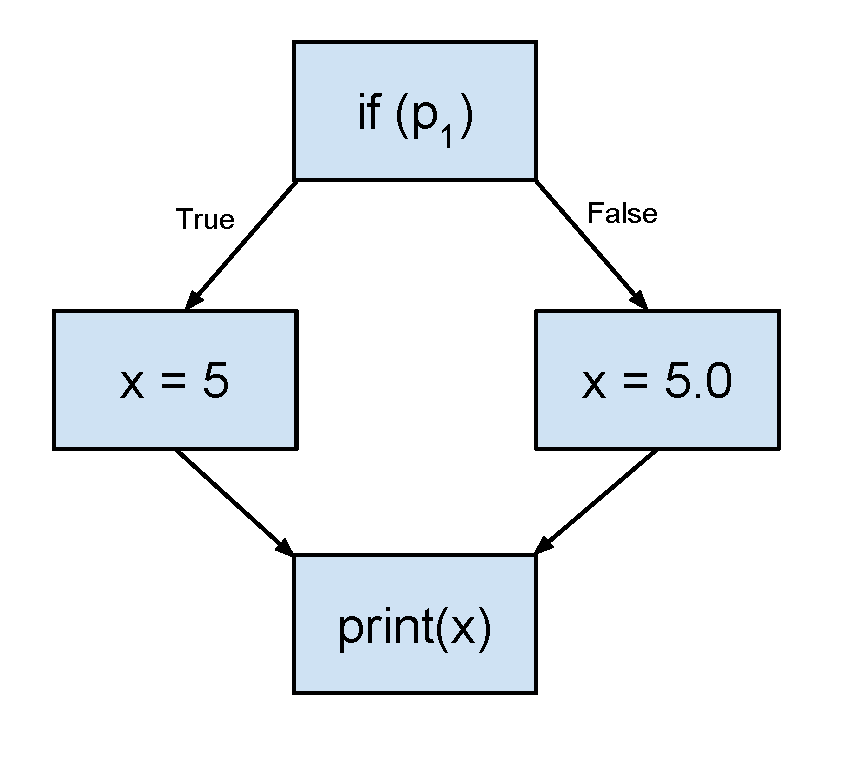
\includegraphics[scale=0.4]{images/controlFlowGraph.pdf}
\end{figure}  \\
Since the primary use for CFGs in computing is for compilers it is natural that a good place to find a CFG generator in Python is in a Python compiler. The most commonly used interpreter for Python code is \textit{CPython}. CPython, which is written in C, uses CFGs~\cite{cpythonCFG}. The CPython process of generating a CFG is to rely on generated bytecode to determine how a program branches on which it is then built. To see the bytecode generated by CPython, consider the following function:
\begin{lstlisting}[mathescape]
    def f():
      return [x for x in range(10)]
\end{lstlisting} 
The generated bytecode in CPython is the following:~\cite{cpythonBytecode}
\begin{verbatim}
    0  BUILD_LIST                     0
    3  DUP_TOP
    4  STORE_FAST                     0 (_[1])
    7  LOAD_GLOBAL                    0 (xrange)
    10 LOAD_CONST                     1 (10)
    13 CALL_FUNCTION                  1
    16 GET_ITER
    17 FOR_ITER                       13 (to 33)
    20 STORE_FAST                     1 (x)
    23 LOAD_FAST                      0 (_[1])
    26 LOAD_FAST                      1 (x)
    29 LIST_APPEND
    30 JUMP_ABSOLUTE                  17
    33 DELETE_FAST                    0 (_[1])
    36 RETURN_VALUE
\end{verbatim}
For the purposes of our application, for function \texttt{f} we need to know that the that we are returning a list comprehension in which \texttt{x} is being assigned the types in the contents of the list being returned by the \texttt{range} function. Learning this information from the bytecode would not be trivial. For instance, the \texttt{RETURN\_VALUE} statement provides the value on the top of the stack as a return type of the function. Without implement an imaginary stack it would not be clear what is being returned. As we can see extracting information from such low-level bytecode is a much more difficult task than from accessing the designated field in the classes of an AST node. For this reason using a CFG built on bytecode presents needless complications. \\
\indent \textit{PyPy}, an alternative interpreter for Python which also uses CFG generation in its tool-chain~\cite{pypyCFG}. Unlike CPython, PyPy is written in Python, however its design is very similar to that of CPython meaning it also depends on a bytecode interpreter to generate its CFGs. \\
\indent In 2013 a student named Ashwin Panchapakesan from the University of Ottawa built a tool to generated CFGs from Python source code~\cite{ashwinCFG}. To do this the program parses an AST created from the Python code into XML. The XML uses tags to indicate the type of a statement, such as if, while or expression. Within these tags is the line number of the statement. The XML format of the program is then analysed in order to determine where each line number is able to flow to. The CFG generated is easy to extract from this program, however the only information contained in this XML are the line numbers making it difficult to work with. While we could just extract the matching lines of raw source code, we would then need to break down the Python syntax ourselves to extract the information to analyse. There is also no simple way to extract the necessary information from the AST based on the line numbers.

\subsubsection{Flow-sensitivity}
A flow insensitive analysis of a program does not consider the order of execution~\cite{nielson99}. That is, each occurrence of a variable typically is represented by the same set of possible types no matter where it appears in the program. Consider the following example:
\begin{lstlisting}
    if (y):	
      x = 5     # S1
    else:
      x = 5.0   # S2
    f(x)        # S3
\end{lstlisting}
A flow-sensitive algorithm would infer the type of \texttt{x} at \texttt{S1} to be $\left\{ {int}\right\}$ and $\left\{ {float}\right\}$ at \texttt{S2}, while a flow-insensitive algorithm would infer the type of $x$ to be $\left\{ {int, float}\right\}$ at \texttt{S1}, \texttt{S2} and \texttt{S3}. \\
\indent Another case in which ignoring the flow of execution can change the types inferred is represented by the following trivial block of code:
\begin{lstlisting}
    x = 5
    x = 5.0
\end{lstlisting}
A flow-insensitive algorithm would infer the type of \textit{x}, for any future occurrences of \texttt{x}, to be in the set $\left\{ {int, float}\right\}$. A flow-sensitive algorithm is able to recognise that the second statement `overwrites' the first. This permits a more accurate representation of the flow, allowing it to infer more accurately the type of \texttt{x} as the set $\left\{ {float}\right\}$. \\
A flow-sensitive algorithm is clearly the more accurate approach but requires a comparatively complex algorithm than a flow-insensitive since the value of variables needs to be tracked at each assignment. \\
\indent Ryder~\cite{ryder03} suggests that the difference between a flow-sensitive and flow-insensitive approach is minimal in regards to object-oriented programs due to the size of methods being small. While Python can be, and is, used for object-oriented programming, a significant number of Python programs are written as scripts and so the benefits of a flow-sensitive algorithm can not ruled out in our case.

\paragraph*{Path-sensitivity}\mbox{} \\
A path-sensitive analysis recognises the path taken at control flow constructs such as \texttt{ifs} and \texttt{whiles} often involve deterministic choices. To exploit this the links between blocks in the control flow graphs are labelled with the condition which needs to met for the transfer of control to take place. The feasibility of this condition in the context of its location in the program is analysed. If the link is deemed infeasible then the link is removed. The result of this procedure is a control flow graph which more accurately represents the program being analysed.

\subsection{SSA Naming}
Primarily used in compilers, Single Static Assignment (SSA) is used to acquire ``unique names for distinct entities.''~\cite{ssaBook} What this means is that each variable should only be assigned to once. There are number of variants of SSA, each designed for a specialised purpose, such as Hashed SSA~\cite{ssaBook} form which intends to capture the fact that a single static use or definition (e.g.\ \texttt{*p} in C) could potentially impact multiple variables. In our case we are only to use a basic version of SSA, `vanilla' SSA which we will now describe. \\
Consider the following example:
\begin{lstlisting}
    x = 5
    y = x + 1
    x = 7
    z = x + 1
\end{lstlisting}
This code violates the SSA requirements since the variable \texttt{x} is assigned to twice. Translating this block into SSA form would give us the following:
\begin{lstlisting}
    x1 = 5
    y1 = x1 + 1
    x2 = 7
    z1 = x2 + 1
\end{lstlisting}
It can be observed that the latest assignment of \texttt{x}  is used in all instances of \texttt{x} where \texttt{x} isn't being assigned a new value. This can be seen in the assignments to \texttt{y} and \texttt{z} where \texttt{x1} and \texttt{x2} is used respectively. \\
Note that the names of, both, \texttt{y} and \texttt{z} need not be changed in this case since they are only assigned to once. However it often makes the implementation of SSA easier to do so regardless.

\subsubsection{The $\phi$ function}
In a sequential program the manner used to number new variables is quite intuitive, we simply increment the number appended the end of the variable name. However as we introduce branching into our programs this method alone breaks down. Consider the following program:
\begin{lstlisting}
    x = 5
    if (y):
      x = 5
    else:
      x = 6
    z = x + 1
\end{lstlisting}
The \textit{if} statement has two branches which both assign a new value to the variable \texttt{x}. Assigning new names to these variables is required by the rules of SSA, however it is unclear which name we are to use after the \texttt{if} and \texttt{else} when \texttt{x} is used in then assignment to the variable \texttt{z}. \\
\indent To resolve this problem, we introduce the concept of the \emph{$\phi$ function}. The $\phi$ function is used ``to merge values from different incoming paths, at control-flow merge points.''~\cite{ssaBook} Put simply, the result of the $\phi$ can be said to be \emph{any} of the parameters given. 
\begin{lstlisting}[mathescape]
    x1 = 5
    if (y):
      x2 = 5.0
    else:
      x3 = 6
    x4 = $\phi$(x2, x3)
    z = x + 1
\end{lstlisting}
Since we only care about the possible types of each variable the $\phi$ function can viewed as a glorified union of all possible types of all parameters in our case. So in the above example we would have $x4 = \phi(x2, x3) = \{Float\} \cup \{Int\} = \{Float, Int\}$. \\
A similar, slightly more complex case arises for loops. In this case, we must consider the types of the variables at each iteration of the loop as well as the exit. Consider the following trivial example:
\begin{lstlisting}
    x = 5
    while (y):
      x = x + 1.0
    z = x + 1
\end{lstlisting}
At the entry of the loop, \texttt{x} can come from the statement immediately before the loop as well as the end of the loop. This can be seen clearly in Figure~\ref{phiCFG} where there are two entries into the loop header where \texttt{x} may take a value. We need to represent the fact that the value of \texttt{x} at the loop header could be either of the values. We do this using the $\phi$ function. The resulting program in SSA form is:
\begin{lstlisting}[mathescape]
    x1 = 5
    x2 = $\phi$(x1, x3)
    while (y):
      x3 = x2 + 1.0
    z = x2 + 1
\end{lstlisting}
The $\phi$ function can also be used for inferring the possible return types of a function. Consider the following Python function:
\begin{lstlisting}[mathescape]
    def f():
        if ($p_1$):
          return 5
        if ($p_2$):
          return "Hi"
        return 5.0
\end{lstlisting}
Here we can see that the function \textit{f} has a number of different \textit{return} statements which can return a number of different types. In order to infer the possible types that a function can return we need to look at the types of each return statements. We can use the $\phi$ function in order to simplify this task. To do so we modify the function as follows:
\begin{lstlisting}[mathescape]
    def f():
        if ($p_1$):
          $r_1$ = 5
        if ($p_2$):
          $r_2$ = "Hi"
        $r_3$ = 5.0
        $r_4$ = $\phi$($r_1$, $r_2$, $r_3$)
\end{lstlisting}

\paragraph*{Creating $\phi$ functions}\mbox{} \\
Since most functions do contain a single set of variables constrained to a single control flow construct but instead have many local variables and many constructs, to create $\phi$ functions we need to know for which variables to create them for. There are two ways we can go about this:
\begin{itemize}
	\item Method One - create a $\phi$ function for every variable within scope.
	\item Method Two - use dominance frontiers to calculate which $\phi$ functions are necessary
\end{itemize}
Method One is very simple to implement. However it clearly comes with some redundancy. It will cause to create $\phi$ functions for variables which are not modified and variables which are no longer referenced in future code. \\
\indent Method Two, dominance frontiers, eliminate redundancy at the expense of a more complicated algorithm. The algorithm is performed on code which has already been transformed into a control flow graph. The algorithm initially determines a \textit{dominance} relationship between the nodes in the CFG. ``Let X and Y be nodes in the CFG. $X$ dominates $Y$ (written $X≥Y$) if $X$ appears on every path from Entry to $Y$.''~\cite{ssaLecture} We extend this to a tighter relationship. We can say that ``$X>Y$ ($X$ strictly dominates $Y$) when $X$ dominates $Y$ but $X \neq Y$.''~\cite{ssaLecture} Using this information we can then begin to compute the dominance frontiers. ``$Y$ is in the dominance frontier of $X$ iff there exists a path from $X$ to Exit through $Y$ such that $Y$ is the first node not strictly dominated by $X$.''~\cite{ssaLecture} Having computed the dominance frontiers we add a $\phi$ function in the dominance frontier of a node for every variable assigned in that node. \\

The usefulness of SSA naming is immediately obvious. We need not track how the types of a variable may change over time. We may treat each new naming as a completely distinct variable. Managing the control-flow also becomes a much simpler task as we are easily able to express the fact that a variable can possibly be a number of different types depending on the path taken through the program.

\begin{figure}[h]
\centering
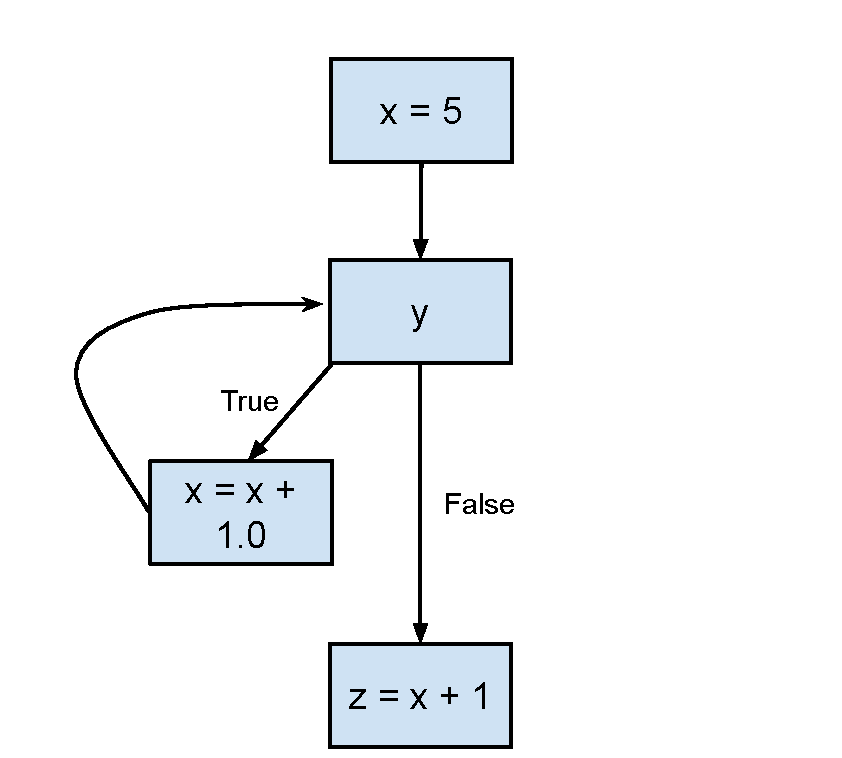
\includegraphics[scale=0.5]{images/ssaPhiNode.pdf}
\caption{while loop as a CFG}
\label{phiCFG}
\end{figure}

\subsection{Dead Code Elimination}
Dead Code Elimination is the process of detecting that a section of code is dead (unreachable) and completely eliminating it from the program. Code may be unreachable if it is placed after a \textit{break}, \textit{continue} or \textit{return} statement or if the code has the effect of only modifying variables which will never be used again (`dead' variables.) The advantages of this is that we need not type check it, thus improving the speed of our program.
An example of this is:
\begin{lstlisting}
   def foo():
   	a = 24
   	b = 25    # Assignment to dead variable
   	c = a + 2
   	return c
   	b = 24 	   # Unreachable code
   	return "Hi"
\end{lstlisting}
We may wish to consider removing dead code from the program in order to type functions more accurately. In the example above, if we did not eliminate dead code we will determine that the return type of the function \textit{foo} as $\{Int, String\}$. Since \textit{Int} is still in the typing, this is not incorrect but a needless overestimate. Dead code also raises some issues in how they should be handled in the CFG. Should \texttt{return c} link to \texttt{b = 24}? However, there is an argument to type checking dead code. This code may become important later and flagging the errors may save the engineer time later on. \\
\indent As well a \texttt{return} statements this problem also applies to \texttt{breaks} and \texttt{continues}. \\
\indent Unfortunately there are no out-of-the-box solutions to this problem for Python programs. \\

\subsection{Constraints and Constraint Solvers}
``A constraint satisfaction problem [CSP] is a problem where one has to find a value for a (finite) set of variables satisfying a (finite) set of constraints.''~\cite{constraintBook} A CSP is typically described using the following notation: $\langle X, D, C \rangle$. Where $X$ represents a set of variables, $D$ is a set of corresponding domains and $C$ is a set of constraints that any solution must satisfy. Every variable must have a \textit{domain}. A domain specifies the values a variable can take. An example domain is the set of integers, $\mathbb{Z}$. A solution to a CSP is a mapping from the given variables to a value in the domain which satisfies the constraints provided. \\
An example of a CSP is the following, where each letter must be replaced with a different number such that the sum evaluates correctly~\cite{constraintPrinciples}: \\
\begin{equation*}
\frac{
    \begin{array}[b]{r}
      SEND \\
      + MORE
    \end{array}
  }{
    MONEY
  }
\end{equation*}
In this problem the  $\langle X, D, C \rangle$ are as follows:
\begin{verbatim}
    X:
      S, E, N, D, M, O, R, Y 
    D:
      [1..9] for S, M
      [0..9] for E, N, D, O, R, Y
    C:
      AllDifferent([S, E, N, D, M, O, R, Y])
      ExactSum([SEND, MORE], MONEY)
\end{verbatim}
Where \texttt{AllDifferent} is shorthand for $S \neq E \neq N \ldots$ and similarly \texttt{ExactSum} is shorthand for $(S \times 1000 + E \times 100 \ldots)  + (M \times 1000 + O \times 100 \ldots) = (M \times 10000 + O \times 1000 \ldots) $ \\
\indent There is a single solution to this CSP:
\begin{verbatim}
    S = 9, E = 5, N = 6, D = 7, M = 1, O = 0, R = 8, Y = 2
\end{verbatim}
Constraints are frequently solved using constraint solvers. A third-party constraint solving package for Python called \textit{python-constraint}. python-constraint provides a number of built-in constraint types to use such as \textit{NotInSetConstraint}, \textit{AllEqualConstraint} and \textit{ExactSumConstraint}. However, it also allows you use a \textit{FunctionConstraint} to which you provide a function defining the constraint logic. This means the constraints it can handle are endless.

\newpage
\section{Type Inference}
The main problem which is required to be solved by this project is how to statically infer the types in Python. \\
\indent In this section we look at a number of the existing techniques to achieve this while keeping in mind the objectives described at the beginning of this report. Those were for it to return a low number of false positives, for it to statically analyse the code (not run it) and for it to be a out-of-the-box solution and for it to be reasonably fast.

\subsection{Hindley-Milner}
The Hindley-Milner algorithm was developed by Robin Milner based on the work of J. Roger Hindley. Hindley described the \textit{principal
type schema}~\cite{hindley69}, ``which is the most general polymorphic type of an expression, and showed that if a combinatorial term has a type, then it has a principal type.''~\cite{cardelli87} Milner's contribution was an extension to Hindley's \textit{principal type schema} which included the ``notion of generic and non-generic type variables, which is essential for handling declarations of polymorphic functions.''~\cite{cardelli87} Milner's work culminated in the type inference system for the ML language~\cite{milner84}. \\
\indent The Hindley-Milner algorithm uses the operations performed on expressions to generate constraints on the types of those expressions. This is done by annotating the nodes of an expression tree with the constraints in a bottom up fashion\footnote{The Hindley-Milner algorithm can be implemented top-down, called the $\mathcal{M}$ algorithm, or bottom-up, called $\mathcal{W}$~\cite{heeren02}. However, the bottom-up version appears to be much more common.}. \\ The constraint is solved to infer a type for a term using a \textit{unification} algorithm.
Bugs can be detected by determining whether there are inconsistencies in the set of constraints.

\paragraph{Limitations}\mbox{}\\
The technique does not allow polymorphic argument to be of a different type in different locations. This is because unification requires there to be a single type for all appearances of a variable. For this reason Hindley-Milner is unable to infer a type for programs such as the following:
\begin{lstlisting}
	if (y):	
	  x = 5     
	else:
	  x = 5.0   
\end{lstlisting}
We have already seen examples such as this in previous chapters, and so the Hindley-Milner approach is not appropriate in our case.

\subsubsection{Pyty}
Developed by Jeff Ruberg~\cite{pyty}, Pyty is a bug checker which analyses annotated source code to detect errors related to the misuse of types. Pyty employs Hindley-Milner as its type inferencing algorithm.
\paragraph{Limitations}\mbox{}\\
Pyty requires annotations to the source code in a specific format. This is quite tedious and prevents from being an `out-of-the-box' solution to our problem.

\subsubsection{Palsberg and Schwartzbach Algorithm}
The Palsberg and Schwartzbach algorithm~\cite{Palsbergstatictyping} works by constructing a network of constraints where each expression in the analysed program is represented by a node in the network. The node contains the types which the expression may assume during execution. All types are initially set to be empty except from constants and literals. The constraints between the nodes are created in response to statements in the program. In the Palsberg and Schwartzbach algorithm there are two ways in which a constraint can generated: assignments and function calls. An assignment such as $x := y$ is represented by the constraint $type(x) \subset type(y)$. Function calls generate constraints between the \textit{actual} arguments used in the function call and the formal arguments in the function definition. The constraints are solved by propagating types through the constraint edges until a fixed-point in reached. \\
\indent The algorithm is used for object-oriented code by copying the bodies of base classes inherited into the child classes. Similarly, class definitions are duplicated at all sites at which they are constructed and method bodies are duplicated at call sites. \\
\paragraph*{Limitations}\mbox{}\\
The excessive duplication makes the algorithm impractical. In the worst case, successive expansions squares the size of the program to be analysed.


\subsection{Cartesian Product Algorithm}
The Cartesian Product Algorithm (CPA) was originally conceived by Agesen as an improvement on the Palsberg and Schwartzbach algorithm for the language Self~\cite{agesen95}. \\
The Cartesian Product Algorithm works by modelling data flow as opposed to the constraint and unification method adopted by the Hindley-Milner algorithm. This is done by building a set of possible types an expression can take. Consider the following code:
\begin{lstlisting}
    if (y):	
      x = 5     
    else:
      x = 5.0  
\end{lstlisting}
The inferred types for $x$ would be the set $\left\{ {int, float}\right\}$, where the possible \textit{int} type is found in the \textit{then} branch and the \textit{float} type is found in the \textit{else} branch. The types from each branch are added to the set of possible types for $x$. The CPA algorithm guarantees that the type of the variable is contained within the set. \\
In order to infer the types handed to a function the cartesian product of the set of possible types for all given arguments is taken. Consider the following code:
\begin{lstlisting}
    if (y):	
      x = 5 
      z = "Hello world"    
    else:
      x = 5.0 
      z = True
    f(x, z)
\end{lstlisting}
The set of inferred types for $x$ is, as before, $\left\{ {int, float}\right\}$ and the set for $z$ is $\left\{ {str, bool}\right\}$. The possible types of the inputs to the function $f$ are: $\left\{ {int, float}\right\} \times \left\{ {str, bool}\right\} = \left\{ {(int, str), (int, bool), (float, str), (float, bool)}\right\}$, where each tuple represents the possible types of the variables given to $f$. \\
The biggest shortcoming of the Palsberg and Schwartzbach algorithm, the expansions, was remedied by the CPA algorithm. This was done by duplicating function bodies such that they contain an argument list with monomorphic types which Agesen calls templates. Each argument list generated by taking the cartesian product at calls sites is connected with constraints to the corresponding template. The types of the values returned by each template are connected to the result of the function call. While duplication still occurs, it is bound the number of possible combinations of the types of the arguments, rather than being duplicated each time for every function call.
\paragraph*{Limitations}\mbox{}\\
The size of the Cartesian products grows exponentially with the number of arguments given to the function call. However the size is bounded by the number of types available. \\
The difficulty of implementation is greater than that of the Hindley-Milner algorithm which is known as being a fairly simple algorithm to implement~\cite{jones95}. \\
Taking the cartesian product of the possible types given to a function call is unnecessary if the possible types the function can take are already known. \\
While duplication has been reduced in comparison to the Palsberg and Schwartzbach algorithm, each function body is still duplicated to generate all possible templates.

\subsubsection{Starkiller}
Starkiller was designed by Michael Salib as a Python-to-C++ compiler~\cite{starkiller}. The type inference of algorithm used was based loosely on Agesen’s Cartesian Product Algorithm and achieves a complete type inference of Python source code.
\paragraph*{Limitations}\mbox{}\\
Starkiller is unable to infer types for the dynamic constructs such as \textit{eval}, or \textit{exec}. Strarkiller does not support exceptions of any kind. The implementation is flow-insensitive and so all variables contain all types inferred at all times. This means Starkiller is not precise. The types of function arguments are inferred from the call sites. This is not a problem since Starkiller is not a bug checker and so the Python source code being analysed, and thus the arguments given to a function call, are assumed to be correct.

\subsubsection{Shed Skin}
Shed Skin is a Python-to-C++ compiler developed by Mark Dufour which boasts up to a 40-fold performance increase over an older Python-to-C++ compiler, Psyco~\cite{shedskin}. Shedskin employs the Cartesian Product Algorithm (CPA) alongside iterative class-splitting. The CPA algorithm is used to allow the user to know which functions need to be defined. For instance, if Shed Skin comes across $max(1, a)$ where $a$ can be the types in the set $\{int, float\}$ the $max$ function needs to be duplicated in C++ to cover $max(int, int)$ and $max(int, float)$ which need to be defined. Dufour also needs to define classes for the types used. For data polymorphic types such as lists, the class cannot always be shared so the the classes are `split' once they can longer share the same representation of data in the equivalent C++ program.

\paragraph*{Limitations}\mbox{}\\
The programs consumed by Shed Skin are required to be implicitly statically typed. Meaning the type of a variable can not dynamically change. Shed Skin also does not support a number of Python features such as \texttt{eval} and \texttt{isinstance}.

\subsubsection{Localized Type Inference of Atomic Types in Python}
For his masters thesis, Brett Cannon attempted to infer the types for local, atomic (built-in) variables are inferred in an attempt to improve the performance of Python~\cite{cannonlocalizedtype}. The type inference is performed by intercepting bytecode from the interpreter and modifying it by injecting additional bytecode relating the the types of variables. The aim is to provide type information which can be utilised to improve performance. Cannon's work differs to Psyco in that the work is done inside Python's compiler, rather than the interpreter.
\paragraph{Limitations}\mbox{}\\
The inference is limited to built-in types: \texttt{integrals}, \texttt{float}, \textit{complex}, \texttt{basestring}, \texttt{list}, \texttt{tuple} and \texttt{dict} so any user-defined types are ignored. \\
\indent The limitations involve only inferring types for local variables, meaning that the implementation is largely useless when used on programs designed with Object Oriented Programming (OOP) in mind, as noted by Cannon. While not a real limitation, Cannon's solution intercepts the compiler in order to improve performance. This is not our aim and we need not complicate things by working with bytecode.

%\subsection{Gradual Typing}


\subsection{Success Typings}
The phrase `success typings' was coined by Lindhal and Sagonas in the 2006 paper \textit{Practical Type Inference Based in Success Typings}~\cite{lindhal06}. The aim of a success typing is to fully describe all possible intended uses of a function. This description is given as type signature for a function $f$: $(\bar{\alpha}) \rightarrow \beta$, where $(\bar{\alpha})$ refers to the type of the function parameters, and $\bar{\alpha}$ is a shorthand for $\alpha_1, \alpha_2,...\alpha_n$, and $\beta$ is the type of the return value. Both types are the `largest' possible types, i.e.\ subtypes are acceptable. For instance, consider the following function as described in the Lindhal et al.\ paper for the functional language \textit{Erlang}:
\begin{lstlisting}[mathescape]
	and(true, true) $\rightarrow$ true;
	and(false, _) $\rightarrow$ false;
	and(_, false) $\rightarrow$ false;
\end{lstlisting}
where the symbol `\_' represents a \textit{don't care} option for pattern matching, meaning it will match any value for the corresponding parameter. \\
\indent An acceptable success typing for this function, and, indeed, for any function with two arguments, would be: $(any(), any()) \rightarrow any()$ where $any()$ denotes the set of all Erlang types. Such a typing would raise no warnings about any use of the function and so can be used when no typing information can be inferred about a function. However, a more useful typing for the function in question is $(any(), any()) \rightarrow bool()$ where the return type of the function is restricted to all subtypes of $bool()$. Since we have the \textit{don't cares} any parameter paired with an instance of $false$, such as $(42, false)$, constitutes a valid use of the function. This optimistic approach avoids any possible false positives and so will never reject a well-formed program. This typing does allow for warnings to be issued as a result of type clashes in matching a value which is not a subtype of $bool()$ with the result of the function. \\
\indent A success typing is inferred by building constraints by traversing the code and then solving them. \\
\indent Constraints are built based on a number of derivation rules. Assume the following definitions: \\
\indent \texttt{e} is any expression which can be defined in the language under consideration, $\tau$ is a type, such as a boolean or integer, \texttt{A} represents an environment with bindings of variables of the form $\{\ldots, x \mapsto \tau_x, \ldots\}$, \texttt{C} represents nested conjunctions and disjunction of subtype constraints, \texttt{V} represents the possible type variables, \texttt{P} represents the set of all possible concrete types and \texttt{T} represents the set of possible types and variable may assume.
\begin{align*} 
	C \coloncolonequals (T_1 \subseteq T_2) \mid (C_1 \land \ldots \land C_n) \mid (C_1 \lor \ldots \lor C_n)
\end{align*}
\begin{align*} 
	T \coloncolonequals none() \mid any() \mid V \mid c(T_1, \ldots, T_n) \mid (T_1, \ldots, T_n) \rightarrow T'\mid T_1 \cup T_2 \mid T \text{ when } C \mid P
\end{align*}
\begin{align*} 
	V \coloncolonequals \alpha, \beta, \tau
\end{align*}
\begin{align*} 
	P \coloncolonequals integer() \mid float() \mid atom() \mid pid()\text{ } | \text{ 42 } | \text{ foo } | \ldots
\end{align*}
and the judgement $A \vdash e : \tau, C$ should be read as ``given the environment $A$ the expression $e$ has type $Sol(\tau)$ whenever $Sol$ is a solution to the constraints in C.'' \\
Then one such derivation rule is the rule for a struct:
                \[
\inference*[STRUCT]{  A \vdash  e_1 : \tau_1, C_1 \ldots e_n : \tau_n, C_n}
                                        {A \vdash  c(e_1, \ldots, e_n) : c(\tau_1, \ldots, \tau_n), C_1 \land \ldots \land C_n}
                \]
The rule states that given a number of elements, each with its own type, can be grouped into a tuple structure in the environment with each individual element retaining their type. The constraints for each element are added to the environment in a conjunction. \\
$Sol$ is a mapping from type expressions and type variables to concrete types. $Sol$ is a solution to a constraint set $C$ if:
\begin{align*} 
	Sol \models T_1 \subseteq T_2 \iff none() \subset Sol(T_1) \subseteq Sol(T_2)
\end{align*}
\begin{align*} 
	Sol \models C_1 \land C_2 \iff Sol \models C_1, Sol \models  C_2
\end{align*}
\begin{align*} 
	Sol \models C_1 \lor C_2 \iff \begin{cases} Sol_1 \models C_1, Sol_2 \models C_2, \\
	                                            Sol = Sol_1 \sqcup Sol_2 \end{cases}
\end{align*}
where $Sol_1 \sqcup Sol_2$ denotes the point-wise least upper bound of the solutions. This means the least general types are taken which satisfies bought $Sol1$ and $Sol2$. The algorithm iterates until this is found. \\
Each case represents a different type of constraint which we may encounter (subtype, conjunction or disjunction). The subtype case states that a solution satisfies a subtype constraint if the mapping satisfies the subtype constraint and neither of its constituents is \textit{none()}. The conjunction case states that the solution must satisfy all conjunctive parts. The disjunction case that the solution is the point-wise least upper bound of all disjuncts.

\subsection{Soft Typing}
Cartwright and Fagan extended the Hindley-Milner $\mathcal{W}$ algorithm to introduce soft typing~\cite{cartwright91}. The aim of soft typing is not to reject a program for which static type checking fails but to ``transform arbitrary programs to equivalent programs that type check.'' Soft typing works by inserting run-time checks, resulting from ``narrowers,'' when a program fails to statically type a program, i.e.\ when unification in $\mathcal{W}$ fails. Narrowers are type casts which blindly convert from the current type to the destination type. Conversion errors are caught by the run-time checks. \\
\paragraph{Limitations}\mbox{} \\
Soft typing requires a program to be run in order to notify the programmer about errors. Our aim is to create a static debugger and so our aims are incompatible with soft typing.

\subsection{Aggressive Type Inference}
Aggressive type inference (ATI) is a technique developed by John Aycock~\cite{aggressiveType} which follows the idea that:
\begin{quote}
	\emph{``Giving people a dynamically-typed language does not mean that they write dynamically-typed programs.''}
\end{quote}
Aycock backs up this hypothesis by citing a study~\cite{typeInferenceIcon} which reveals that around 80\% of operators in a set of \textit{Icon} programs maintain the same type throughout their lifetime. \\
\indent He exploits this by using a flow-insensitive method and does not use union types. Meaning the algorithm does not look through all routes to determine all possible types for a variable and only labels a variable with a single type, not a union of multiple types. The algorithm works by iteratively analysing the code to infer the types of variables and by propagating the types on each iteration.
\paragraph{Limitations}\mbox{}\\
The limitations of Aycock's approach are quite clear: the types involved in dynamic behaviour are not reliably extracted. How much of an issue this poses is up for debate;
A study on this, more recent and relevant to our interests than the \textit{Icon} analysis put forward by Aycock, has been conducted by Alex Holkner and James Harland~\cite{evaluatingDynamicBehaviour}. This study details the evaluation of twenty-four open source Python systems. Their results argue that dynamic features are actually widely used. For instance, they find that all systems studied employ dynamic code execution. Holkner and Harland concede that their study is small in comparison to the amount of Python code available, however if their results are to be extrapolated then Aycock's assumption is not so reasonable.

\subsection{RPython}
RPython is an intermediate language, a subset of Python which is entirely statically typed and which acts as a link in the PyPy toolchain. PyPy's goal is to develop a Just-In-Time (JIT) compiler for Python. PyPy's interpreter is written in RPython which removes dynamic features in order to reduce the complexity of type inference.
\paragraph{Limitations}\mbox{}\\
The major limitation of PyPy is the use of RPython. One feature of RPython is that it does not allow variables to change their type.

\subsection{Related Work}
To the best of my knowledge, there is currently no bug finder for type errors in Python which does not return any false positives. The most active debuggers at the time of writing are Pylint and and PyChecker.
%\subsubsection{Psyco}
%Psyco is a just-in-time (JIT) compiler for Python, designed to improve performance~\cite{psyco}. Psyco replaces the main interpreter loop of Python in order to examine the bytecode and, where appropriate, emits specialized bytecode in its place. CITATION NEEDED
%\paragraph*{Limitations}\mbox{}\\
%Psyco only attempts to infer locally defined \textit{ints} and \textit{strings} and pays little interest to any other types.

\subsubsection{Pylint}
Pylint is an error checking tool for Python which statically analyses Python source code to look for errors, including type errors, and to assess the coding style. Pylint is a static analyser and so it looks for errors without running the source code. \\
\indent Documentation on Pylint is almost non-existent and the source code is also quite difficult to understand so, unfortunately, we currently do not understand the type inference algorithm of Pylint.
\paragraph{Limitations}\mbox{}\\
Can often return a lot of false positives and offers a large number of command-line options in an attempt to allow users to manually suppress them.

\subsubsection{PyChecker}
PyChecker is an bug checker for Python which checks for type errors among a host of other errors. PyChecker is similar to Pylint except it does not checker the coding style of the source program. PyChecker also differs in that it needs to runs the code in order to analyse it.
\paragraph{Limitations}\mbox{}\\
The type inference is quite limited. PyChecker focuses on 'softer' type errors, such as whether a variable exists and whether self is the first method argument. \\
PyChecker can return spurious errors and warnings. PyChecker imports the code it is analysing which, due to the fact this execute top-level code, can have undesirable side effects, such as executing a database query in the code.

\subsubsection{PySonar}
PySonar was developed by Yin Wang while an intern at Google between 2009 and 2010 and was intended for the internal use within Google's Grok project~\cite{pySonar}. PySonar was primarily developed as a tool to allow the user to better search and understand Python code. It includes a type inferer in order for the types of variables to be displayed in a tooltip. It also includes an indexer to allow quick search through code. PySonar uses abstract interpretation to infer the types of the variables. PySonar claims to be able to resolve the names of 97\% of the Python standard library.
\paragraph{Limitations}\mbox{}\\
PySonar is focused on indexing the code it analyses and so it does not report any possible type errors. The program focuses mainly on a less dynamic subset of Python which is `easier' to analyse.

\subsubsection{Pyntch}
Created by Yusuke Shinyama, Pyntch uses type inference in Python in order to find bugs~\cite{pyntch}. The method used is `type flow analysis', which is a form of a data flow analysis where the types are tracked as they flow from variable to variable. \\
Project activity has ceased since 2009.
\paragraph{Limitations}\mbox{}\\
Pyntch completely disregards execution order. In the following example given by the author:
\begin{lstlisting}[mathescape]
	x = 1
	x = 'a'
\end{lstlisting}
The variable \textit{x} will always have the type $\{int, string\}$ after analysing the second statement. \\
Pyntch is unable to infer types in code which use the following functions: globals, locals, getattr, setattr, eval, compile or exec. \\
As well as the inaccuracies listed, the Pyntch author states that ``sometimes Pyntch brings a lot of false positives in its result, which need to be further examined by human programmers.''

%\subsection{Javascript}
%Javascript is a dynamically typed scripting language, similar to Python. \\
%Abstract interpretation lattice \\


\subsubsection{Ruby}
Ruby is a dynamically typed scripting language, similar to Python. \\
Furr et al. developed Diamondback Ruby (DRuby)~\cite{furr09} in order to discover type errors. DRuby works by using type annotations of library functions in order to generate constraints to infer the types for user defined functions. DRuby is an aggressive error checker and so reports false positives. \\
\indent An extension to Diamondback Ruby, $\mathcal{P}$Ruby, was created in order to handle difficult dynamic language constructs such as the \textit{eval} method which converts a string into executable program code.~\cite{pRuby} This is done by instrumenting the code such that, when the program is run, all uses of the dynamic constructs are recorded. This allows a \textit{profile} to be built which fully describes how they were used. With this profile the dynamic code can be inserted into the program in place of the dynamic constructs. The modified program can then be statically analysed just like any other. Furr et al. use DRuby for the analysis. Since this process involves running the code it offers no real solution to this problem in regards to static analysis.











\newpage
\section{Implementation}
All of the implementation was created using the language Python. This was decided purely due to the the built-in \texttt{ast} module which provided the base from which this project was built. Since no other language offered such a critical component out-of-the-box this was an easy decision. \\
\indent Our project uses a flow-sensitive approach. This was decided in order to increase accuracy. To implement flow-sensitivity, we use single static assignment. \\
\indent The basic structure of our system can be seen in Figure~\ref{fig:systemStructure}. The basic components are the AST, CFG, SSA, Preprocessing and Type Inference. Each component will be described here. \\
This traverser used to navigate the AST are taken from Edward K. Ream's \textit{stc}~\footnote{\url{https://code.launchpad.net/~edreamleo/python-static-type-checking/trunk} Revision \#448 was used for this project.}. \\


\begin{figure}
\centering
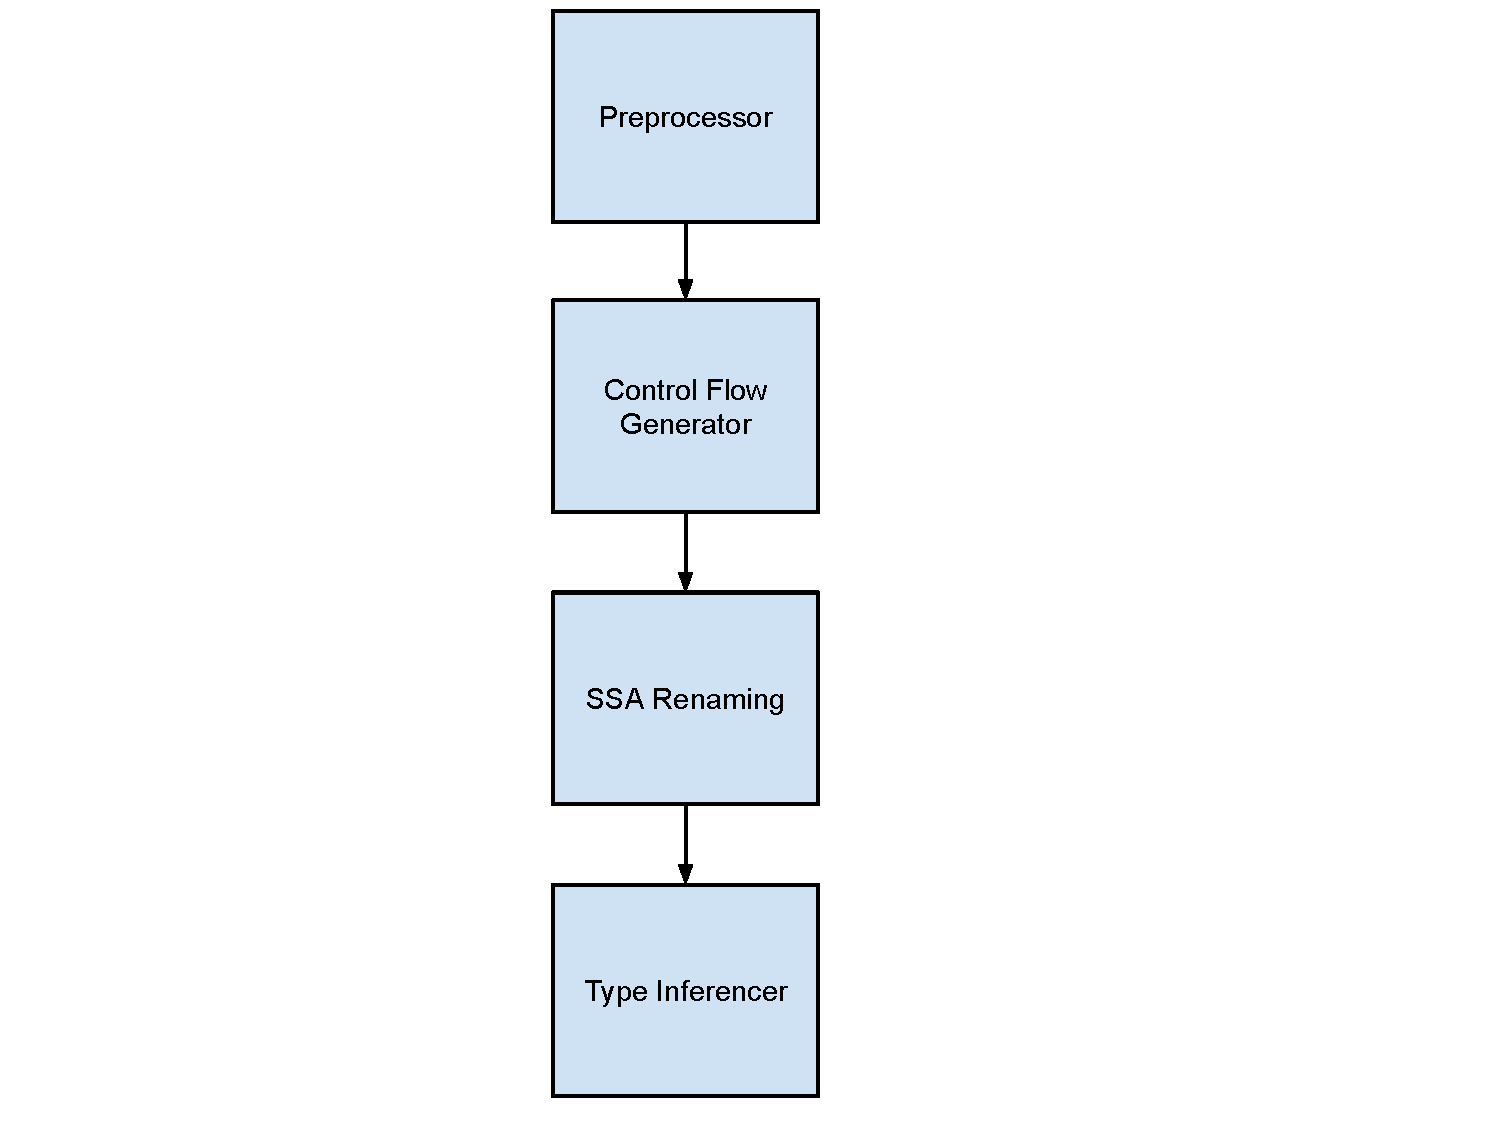
\includegraphics[scale=0.5]{images/systemStructure.pdf}
\caption{Each box represents a key component of the system. Arrows represent the flow of information from each component to another.}
\label{fig:systemStructure}
\end{figure}

\subsection{Preprocessing}
The preprocessing step is designed to modify the AST generated by the \texttt{ast} module in order to simplify the further steps. Some information extraction is also performed, such as the context of each node and the list of global variables in modules and classes are calculated.

\subsubsection{\textit{with} statements}
When dealing with objects which need to be built up before their use and clean up after they have been used, such as file manipulation, engineers using Python had to follow a process similar to the following in the past:
\begin{lstlisting}[mathescape]
	# Set up object
	file = open("file.txt")
	try:
		# Do something
		data = file.read()
	finally:
		# Clean up
		file.close()
\end{lstlisting}
The code ensures the the object is constructed before use, due to flow restrictions, and destroyed after being used since all paths exiting the \textit{try} must lead to the finally. Python 2.5 introduced the \textit{with} keyword to make this code cleaner. Using \textit{with} a example on a file becomes:
\begin{lstlisting}[mathescape]
	with open("file.txt") as file:
		data = file.read()
\end{lstlisting}
\textit{with} works by calling the \textit{\_\_enter\_\_} function on the object provided immediately after the \textit{with} keyword (\textit{open} returns a file) and calling the \textit{\_\_exit\_\_} function when the body has exited. An engineer can build their class to work with the \textit{with} keyword by implementing these functions with their construction and destruction code. For example:
\begin{lstlisting}[mathescape]
	class Example():
		def __enter__(self):
			pass
			
		def __exit__(self, type, value, trace):
			pass
			
		def do_something(self):
			# Do something
			
	with Example() as ex:
		ex.do_something()
\end{lstlisting}
The \textit{type}, \textit{value} and \textit{trace} parameters provide information which can used to handle exceptions. \\
We can handle the \textit{with} keyword by de-sugaring it back into its equivalent try-finally. The set-up code will involve assignment to the specified variable and a call to the \textit{\_\_enter\_\_} function. The finally block will simply consist of a call the \textit{\_\_exit\_\_} function. Our transformed \textit{with} using the \textit{Example} class will look like so:
\begin{lstlisting}[mathescape]
	ex = Example()
	ex.__enter__()
	try:
		ex.do_something()
	finally:
		ex.__exit__(p1, p2, p3)
\end{lstlisting}
The main difficulty involved with this transformation is simulating the variables passed to the \textit{\_\_exit\_\_} function. The simplest way to deal with this is to pass temporary variable which have an \textit{Any\_Type}.

\subsubsection{Augmenting Assignments}
An augmenting assignment performs a binary operation and a store operation on a variable in a single statement. The benefit to using an augmented assignment rather than the two-statement equivalent is three-fold. An increase in clarity of the intentions of the programmer, a reduction in code size and a possible performance boost. The increase in performance arises from being able to express that ``the left-hand operand in question [\ldots] should operate `on itself', rather than creating a modified copy of itself.''~\cite{pepAugAssign} Assuming the Python interpreter is not able to catch this. \\
\indent To deal with augmenting assignments in our type inferencer we simply convert the augmenting assignments into regular assignments with the the binary operation equivalent. The different binary operators permitted in augmenting assignments and how they are transformed can be seen in Table~\ref{table:augAssign}. This transformation saves us from having to repeat the same logic for augmenting assignments that is already present in regular assignments and binary operations.

	\begin{table}
	\centering
    \begin{tabular}{ | c | c |}
    \hline
    \textbf{Original Expression} & \textbf{Transformed Expression}  \\ \hline
    $x \: +\!= y$ & $x = x + y$   \\ \hline
    $x \: -\!= y$ & $x = x - y$   \\ \hline
    $x \: *\!= y$ & $x = x * y$   \\ \hline
    $x \: /\!= y$ & $x = x / y$   \\ \hline
    $x \: \%\!= y$ & $x = x \: \% \: y$   \\ \hline
    $x \: *\!*\!= y$ & $x = x *\!* \: y$   \\ \hline
    $x \: \ll = y$ & $x = x \ll y$   \\ \hline
    $x \: \gg = y$ & $x = x \gg y$   \\ \hline
    $x \: \&\!= y$ & $x = x \: \& \: y$   \\ \hline
    $x \: \wedge\!= y$ & $x = x \wedge y$   \\ \hline
    $x \: |= y$ & $x = x \: | \: y$   \\ \hline
    \end{tabular}
    \caption{The different transformations made to augmenting assignments involving two variables, $x$ and $y$.}
	\label{table:augAssign}
    \end{table}

\subsection{Generating the Control Flow Graph}
Due to the limitations of the CFG generators for Python as previously described, the decision was made to create our own. It was felt that no current generator provided a platform to extract a CFG containing the necessary information about each statement which wouldn't require time consuming modification. The benefit of writing our own generator was that it could be written in a manner which will make it easy to integrate with the design of the SSA and type inferencer. We create CFGs for functions only.

\subsubsection{Ifs and Elses}
For \texttt{if} nodes we add the test to the current block. A new block is each created for the \texttt{then} and \texttt{else} bodies to be used as their initial blocks. These new blocks are set as the current block before each bodies are processed. A block is created as an `exit' node and the last active blocks in each of the \texttt{then} and {else} block are linked to the exit node. An \texttt{if} with a \texttt{then} and no \texttt{else} is legal Python. In this case the block containing the \texttt{if} is linked the `exit' block in place of the initial \texttt{else} block. These can be seen in Figure~\ref{fig:ifcfgs}.

\begin{figure}[t]
    \centering
    \begin{subfigure}[t]{0.5\textwidth}
        \centering
        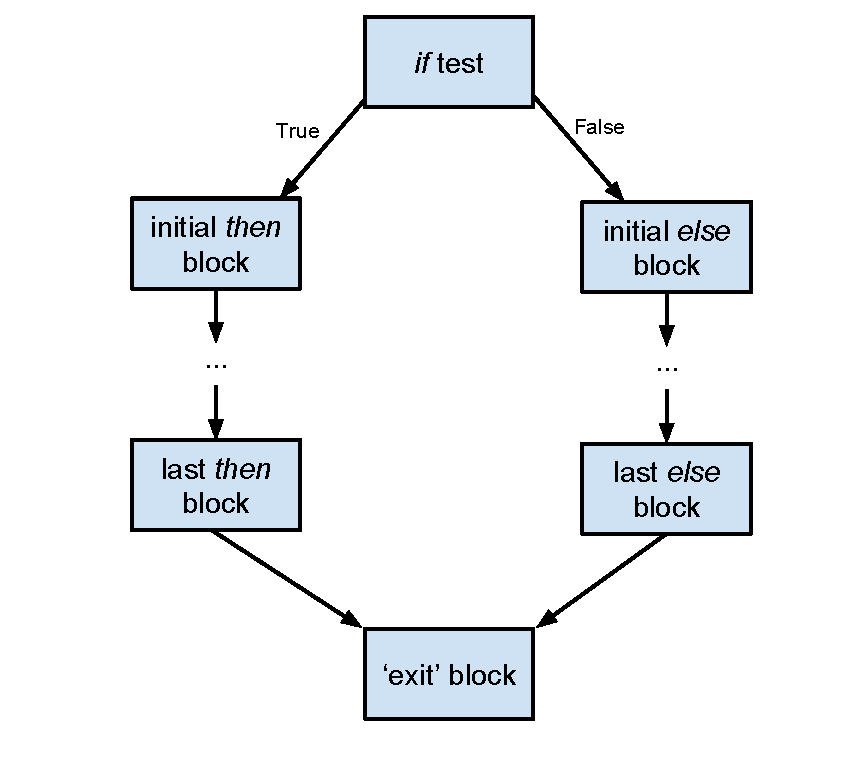
\includegraphics[scale=0.6]{images/cfgIfthenelse.pdf}
        \caption{A general CFG created for an \texttt{if-then-else}.}
    \end{subfigure}%
    ~ 
    \begin{subfigure}[t]{0.5\textwidth}
        \centering
        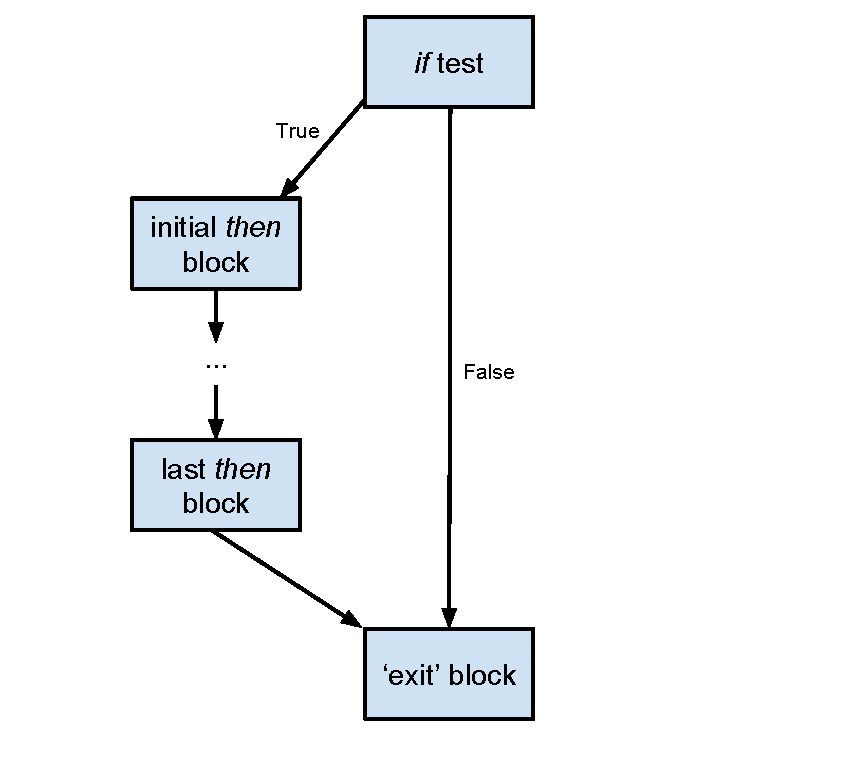
\includegraphics[scale=0.6]{images/cfgIfthen.pdf}
        \caption{A general CFG created for an \texttt{if-then}.}
    \end{subfigure}
    \label{fig:ifcfgs}
    \caption{The cases for CFG generation for \texttt{if} statements.}
\end{figure}



\subsubsection{For and While Loops}
For the purposes of our control flow graph generation \texttt{for} and \texttt{while} loops are the same and so are dealt with in the same manner. The process is similar to that of the \texttt{if}.  We create a new block as the initial block for the body of the loop. However, the loop test is given a block to itself and the last block to be active at the end of the loop body is linked the the test block rather than the `exit' block. \\
\indent Python allows an \texttt{else} block to be added the end the loop. An example of this is as follows:
\begin{lstlisting}
    for entry in some_list:
      if entry == some_i_want_to_find:
        found = entry
        break
    else:
      found = special_not_found_value
\end{lstlisting}
The \texttt{else} body is only entered if the loop test evaluates to \texttt{False}. In the case of \texttt{for} loops reaching the end of the specified iteration is equivalent to \texttt{False}. The \texttt{else} block is not entered when a \texttt{break}, \texttt{exception} or a \texttt{return} occurs. \\
\indent In the case of an \texttt{else} being present the loop test links to the initial \texttt{else} block and the last block in the \texttt{else} to the `exit' block. Otherwise the test links to the `exit' block.

\paragraph*{Breaks and Continues} \mbox{} \\
Taking inspiration from the CFG generation in PyPy, a stack was implemented on which labels are pushed alongside their corresponding nodes. When we reach a loop definition we push a \texttt{F\_BLOCK\_LOOP} onto the stack. Once we encounter a \texttt{break} or a \texttt{continue} statement we cycle through the labels until we encounter the top-most \textit{F\_BLOCK\_LOOP} label. Then for a \texttt{break} statement we add an exit for the current block to the loop's `exit' block. For a \texttt{continue} statement we link the current block to the loop block itself .

\subsubsection{Try, Excepts and Finallys}
The \texttt{try} keyword can be used in a few different ways in Python. Firstly it can be used to catch exceptions to prevent the program crashing, much like in Java. Also like Java, different exceptions in the same try block can be caught and dealt with separately. Consider the following example:
\begin{lstlisting}
    try:
      if some_condition:
        open("myfile.txt")
      else:
        x = 5 / y        
    except IOError:
      # Deal with error
    except ZeroDivisionError:
      # Deal with error
\end{lstlisting}
The statement \texttt{open("myfile.txt")} will lead to the \texttt{IOError} except block if, for instance, the file does not exist. The \texttt{x = 5 / y} will lead to the \texttt{ZeroDivisionError} if \texttt{y} is equal to \texttt{0} at the time of execution. In order to accurately create a control flow graph for \texttt{try} and \texttt{excepts} we need to know which statements can create exceptions and which exceptions they can create. While very time consuming, this knowledge can be gathered from the builtin exceptions and statements in the Python language and standard library and then hardcoded into our CFG generator. But Python permits the creation of unique exceptions by creating a class which inherits from the builtin \texttt{Exception} class. This would be very difficult to track. For this reason the design decision was made to attempt to minimise any false positives. This was done by determining that every statement in a \texttt{try} block can lead to every \texttt{except} block. \\
\texttt{try}s can also be used to ensure that a particular block of code is always executed. This done by using the \texttt{finally} keyword. All code in the \texttt{finally} block is executed no matter how the \texttt{try} body is exited. Normally \texttt{finallys} are used for clean up code. For example:
\begin{lstlisting}
    try:
      file = open(filePath, 'w')
      file.write("something")
    finally:
      file.close()
\end{lstlisting}
\indent Nested \texttt{finally}s are all executed no matter where an \texttt{exception}, \texttt{return} or \texttt{break} occurs. For instance if the following is executed:
\begin{lstlisting}
    try:
      x = 1
      try:
        return
      finally:
        print("finally 1")
    finally:
      print("finally 2")
\end{lstlisting}
Then ``finally 1'' and ``finally 2'' will be printed in that order. \\
\indent \texttt{finallys} and \texttt{excepts} can be used together. In this case the relevant \texttt{except} block is executed first and then passes control to the finally block. \\
\indent If a \texttt{try-finally} is within a \texttt{try-except} then exceptions raised still lead to the \texttt{finally} before passing control to the outer \texttt{except} block. For example:
\begin{lstlisting}
    try:
      x = 1
      try:
        raise Exception
      finally:
        print("finally")
    except:
      print("except")
\end{lstlisting}
In the above example after the exception is raised then ``finally'' and ``except'' are printed in that order. \\
\indent Naturally Python provides a way for the \texttt{else} keyword to be used in conjunction with \texttt{trys}. The \texttt{else} block is executed after the \texttt{try} body providing no exception is raised. This is typically used in cases where one action is to be taken for exceptional execution and another for non-exceptional execution. For example:
\begin{lstlisting}
    try:
      result = 1 / f(x)
    except ZeroDivisionError:
      logging.info('Infinite result')
    else:
      logging.info('Finite result')
\end{lstlisting}
When an \texttt{else} is used in conjunction with a \texttt{finally} then the \texttt{else} body is executed before the \texttt{body} of the \texttt{finally}.

\subsubsection{Wrapping exit blocks}
At the end of the programming constructs dictating control flow a new block is created as an `exit' block to which the blocks exiting the construct (such as a \texttt{break} in a loop) are linked to. However a problem arises when constructs are nested. Consider the following:
\begin{lstlisting}
    if c1:
      # First then block
      if c2:
        # Second then block
      else:
        # second else block
    else:
      # Second else block
    # exit
\end{lstlisting}
The exit block for the inner \texttt{if} is not needed as there no further statements in the first \texttt{then} body. Instead the exit block for the inner \texttt{if} should be the same as the outer \texttt{if} as exiting each one will lead to the same. Thus we need to wrap the inner exits up a level such that they point to the correct location. To ensure this occurs we check the last active block once each path has been analysed. If the block is not empty then proceed as normal. If the block is empty we delete the block and update the reference to point to the exit block for the current construct.

\subsection{SSA Form}
The implementation of SSA renaming was performed precisely as described in the background section. A few additional allowances were required for the system to function correctly. These will be explained here. \\
\indent Having created the CFG our SSA naming can ignore specifics programming constructs such as \texttt{for}, \texttt{if} and \texttt{while}. The knowledge required to successfully create the phi-nodes are encapsulated for these constructs are encapsulated in the exits for each basic blocks in the CFG. \\
\indent The algorithm works by analysing each function at a time. A dictionary is held with each variable name eligible within the current scope. The dictionary is reset to containing only module/class wide variables at the end of each function. When a identifier is encountered it is determined whether we wish to rename it. If we do then we check whether it is a \texttt{store} or \texttt{load} operation. A \texttt{store} checks whether the identifier has been referenced beforehand. If hasn't we add the identifier to the dictionary along with the value \texttt{1} and modified by appending that value. Otherwise the identifier's value is incremented and renamed with the new value. A \texttt{load} operation uses the latest the latest value for that identifier. Once we reach the end of a basic block the state of current block's dictionary is forwarded to all of the block's exits.

\subsubsection{Global and Local Variables}
We consider a global variable to be a variable in the Module-wide or Class-wide namespace. This includes all imports, function identifiers and all of the built-in functions and classes. A local variable is one which is limited to the scope of a function. \\
Consider the following snippet of Python code:
\begin{lstlisting}
    class C():
      def f(self):
        self.x = 5
     
      def g(self):
        self.x = 5.0         
        
      def h(self):
        a + self.x 
\end{lstlisting}
The references to $self.x$ refer to the same variable. The principles of SSA naming state that a variable should only be assigned to once. But which $x$ should be labelled $x_1$ and which should be labelled $x_2$? Or, rather, which of the assignments to $x$ in function \textit{f} and function \textit{g} will be called first? Without any analysis of the call sites or typical run-time behaviour it is impossible to determine this statically. A similar problem arises when we attempt to decide which reference to give to the instance of \textit{self.x} in function \textit{h}. Without knowledge of the order the functions are called (if a consistent ordering even exists) we cannot predict which is the correct label. For this reason SSA naming is only performed on local variables. \\
Separating which variables are global and which are local is not simple due to the fact it can change line-by-line.

\paragraph*{Global Keyword}\mbox{} \\
The keyword \texttt{global} in Python is used to enable the programmer to write to the global namespace within a function. By default the programmer has immediate read access to the global scope and read/write access to the local scope. This means the \texttt{global} keyword is only necessary when a write to the global scope is to take place within the function. With the keyword global variables and global functions can be defined dynamically at runtime. If an identifier to a global variable is modified without indicating this with the \texttt{global} keyword then a new local variable with the same name is created. Consider the following code:
\begin{lstlisting}
	x =  5
    def f():
      x = "Hi"
      y = x
      
      
    def g():
      global x
      x = 5.0
      y = x
\end{lstlisting}
Function \texttt{f} does not modify the global variable. Instead a local variable is created. In the rest of the function \texttt{x} will reference the local variable created. The global \texttt{x} cannot be accessed unless a highly dynamic method is used, such as \texttt{globals().get("x")} where the function \texttt{globals} returns a dictionary containing all global variables. \\
It is common in Python to use the \texttt{global} keyword at the beginning of the function to increase clarity, however Python code in which the global keyword is used \textit{after} the variable has been assigned functions correctly, i.e.\ $x$ in the global namespace is assigned the value (despite the Python interpreter issuing a warning to the programmer.) Therefore we need only worry if the a variable name is used in conjunction with the keyword \textit{somewhere} in the function. \\
Using this knowledge every time a global variable is edited inside of a function we begin the SSA naming unless the identifier is inside of a list of variables which are used in conjunction with the \texttt{global} keyword at some point in the function. For example:
\begin{lstlisting}
	x =  5
    def f():
      y = x
      x1 = "Hi"
      y = x1
      
     
    def g():
      global x
      x = 5.0
      y = x
\end{lstlisting}
In function \texttt{f} the global keyword is not used with \texttt{x} and so we perform SSA on the variable whereas in function \texttt{g} it has been used and so we the identifier is not renamed.

\subsection{Type Inference}
Type inference in our system works by creating a network modelling the data flow of types. The inference works by propagating primitive types through the constraints until the system has been completely satisfied. The primitive types supported by this system are:
\begin{itemize}
	\item \texttt{int}
	\item \texttt{float}
	\item \texttt{bool}
	\item \texttt{bytes}
	\item \texttt{string}
	\item \texttt{list}
	\item \texttt{tuple}
	\item \texttt{dict}
	\item \texttt{set}
	\item \texttt{generator}
	\item \texttt{none}
	\item \texttt{module}
	\item \texttt{class}
	\item \texttt{function}
\end{itemize}
All but \texttt{int}, \texttt{float} and \texttt{bytes} have builtin functions which can be called. These are supported, as far has been deemed productive and necessary, and the complete list can be seen in (appendix - to do). On top of these types we make use of a special type, \texttt{any} which represents the fact the variable could be any possible type and as such is permitted in all circumstances. \\
\indent Initially a pass over the entire program is made and every variable encountered is initialised to an empty type variable. Each context in the program has a mapping of the name of every variable accessible in the current scope to its corresponding type variable. In the case that access of variable is permitted in more than one scope, the corresponding type variable is passed from the parent context to the child.

\subsubsection{Inferring the Types of Simple Assignments}
All changes to the types of variables involve assignment. For each assignment the variable on the left-hand side (LHS) assumes all of the types which the right-hand side (RHS) can possibly have. The following shows a number of ways in which this can be done.
\begin{lstlisting}
	x = 5
	y = x
	z = f()
\end{lstlisting}
 If the RHS is a function then we assign all of the types the function can possibly return. \\
\indent We simulate this flow of types with a simple subset relationship. The set of types the RHS can assume must be a subset of the set of types the LHS can assume. \\
Python allows assignment to variables to be performed inside of lists or tuples. For example:
\begin{lstlisting}
    (x, y) = (1, 1.0)   # 1
    [x, y] = [1, 1.0]   # 2
         x = (1, 1.0)   # 3
         x = [1, 1.0]   # 4
\end{lstlisting}
In the first and second cases \texttt{x} is assigned an \texttt{int} type and \texttt{y} is assigned a \texttt{float} type. However in the third and fourth cases we want to assign a \texttt{tuple} and \texttt{list} type to \texttt{x} respectively. \\
Python also supports double assignment such as the following:
\begin{lstlisting}
    x = y = 5
\end{lstlisting}
This is equivalent to \texttt{x = 5; y = 5} rather than \texttt{x = 5; y = x}. For local variables this we would not be able to distinguish the difference to SSA. However for global variables this would result in a over-approximation.

\begin{figure}
\centering
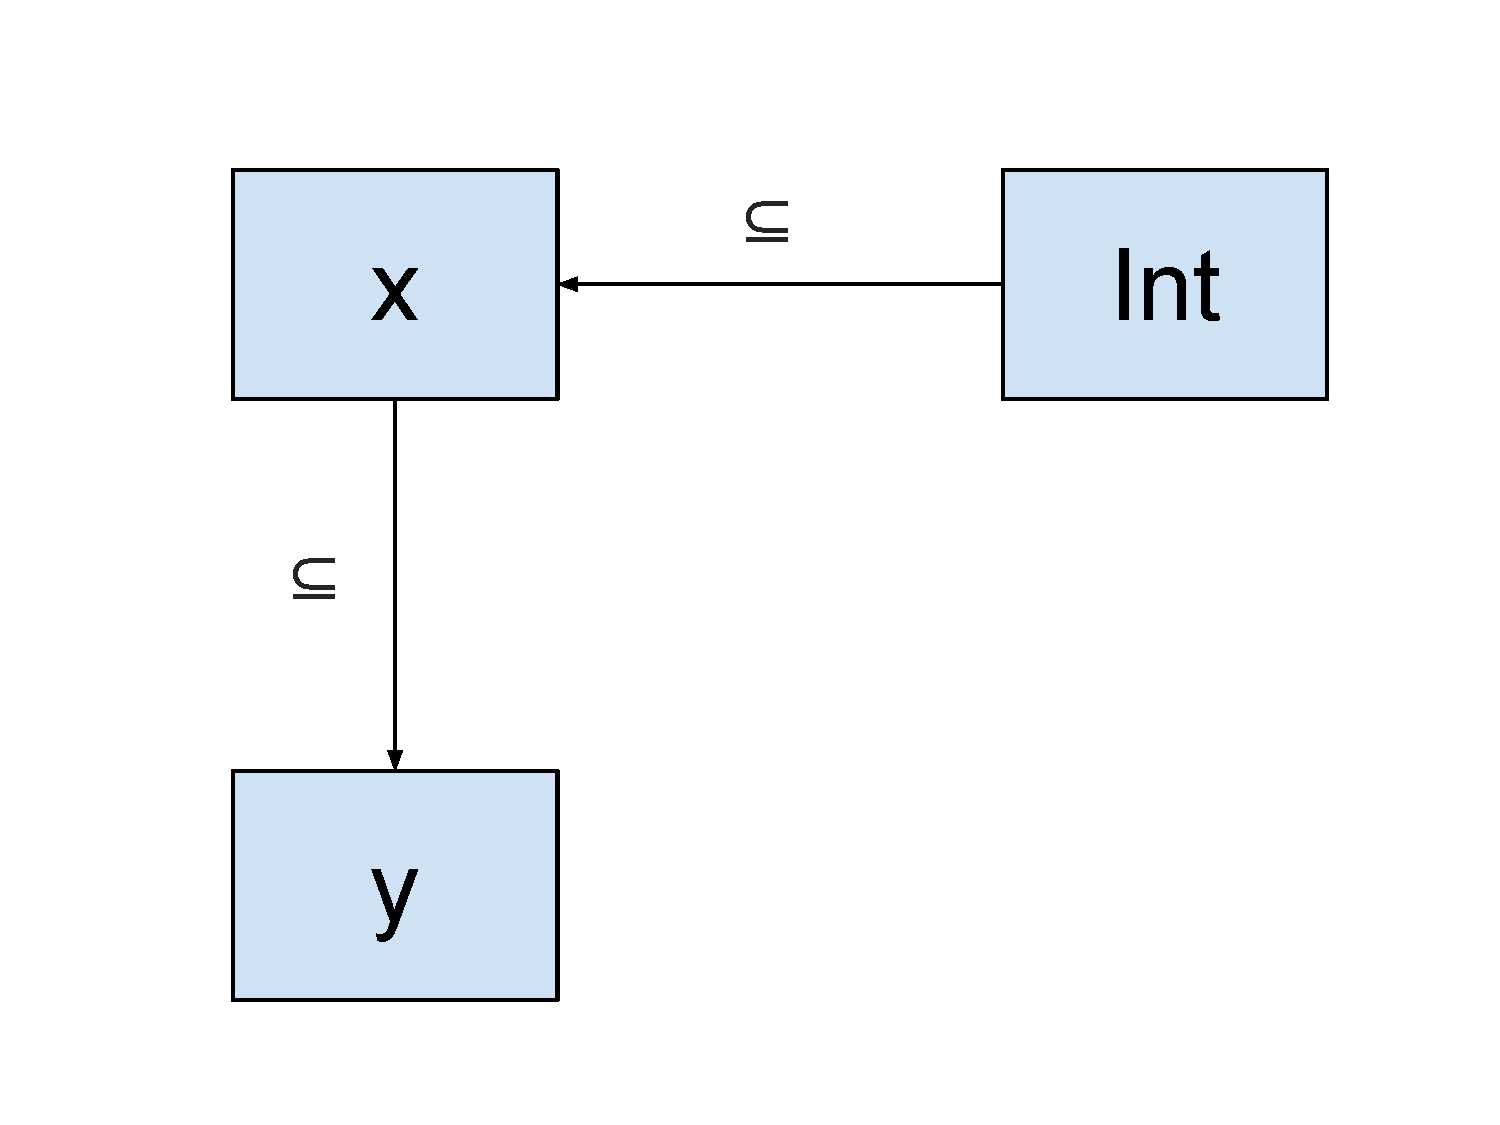
\includegraphics[scale=0.3]{images/assignment_constraint.pdf}
\label{figure:assignConstraint}
\caption{The constraint network generated by the assignments, \texttt{x = 5} and \texttt{y = x}.}
\end{figure}

\subsubsection{Inferring the Types of Binary Operations}
Binary operators are handled by our type inferencer by first inferring the types of the left and right hand side of the operator. We then determine whether there is at least one combination between the two sets of types which can be legally used with the operator. \\
A comprehensive list of the binary operators and the types which can be legally used in combination with them can be seen in Appendix~\ref{App:AppendixBinary}


\subsubsection{Inferring the Types of Unary Assignments}
Python has a small number of unary operators. These are all numeric operators, such as the bitwise not, $\sim$, aside from the boolean operator \texttt{not}. The numeric operators can only be applied to \texttt{ints} and \texttt{floats}, however the \texttt{not} operator can be legally applied to any type.

\subsubsection{Inferring the Types in a `Container' Type}
By a `container' we refer to any type which can contain other types. In the builtin types these are \texttt{list}, \texttt{dict}, \texttt{set} and \texttt{tuple}. \\
\indent Types can be added to these container typically through indexing and using functions. For example, using a list:
\begin{lstlisting}
    x = []
    x[0] = 5        # Indexing
    x.append(5.0)   # Using a function
\end{lstlisting}
No container in Python is restricted to any one type. In the example above the \texttt{list} \texttt{x} contains the types $\{$\texttt{int}, \texttt{float}$\}$ after the function \texttt{append} has been called. In the case of \texttt{dict} which is mapping of key/values it is not limited in the types it contains for keys or values. For instance a single \texttt{dict} instance could contains mappings from \texttt{strings} to \texttt{ints} and \texttt{floats} to \texttt{lists}. \\
\indent All of these container types, aside from \texttt{tuple}, are \textit{mutable}. A type type is considered mutable if value of type's object instance is liable change. An \textit{immutable} type's object value is not liable change to chance once it is created~\cite{pythonMutable}. The effect of this is the following:
\begin{lstlisting}
    def f(y):
      y.append("mutable")
     
    def g(y):
      y = 5.0
      
    x = [5]
    f(x)
    print(x)    # prints [5, "mutable"]
    
    x = 5
    g(x)
    print(x)    # prints 5
\end{lstlisting}
The \texttt{int} type is immutable and so the function can in now way edit the value of \texttt{int} object. Since the \texttt{list} is mutable the function call was able to change the contents of the list and therefore the types contained in the list. What this means in the context of the type checking is that if we wish to accurately track the possible types of the contents of a container type then we must also keep track of the possible side-effects of functions. In the case above we must express that the function \texttt{f} will always add the type \texttt{string} to its first (and only) parameter. When the function is called we must update the possible types the \texttt{list} can contain. So for example, using SSA:
\begin{lstlisting}
    def g():
      x1 = [3]
      f(x1)
      x2 = __side_effects(f, x1)
      print(x2)
\end{lstlisting}
where \texttt{\_\_side\_effects} performs whatever the changes the function has on the contents of \texttt{x1}. The same must also be done for the builtin functions, such as \texttt{append} for \texttt{list} which adds the parameter to the list. \\
\indent Unfortunately this process is either all-or-nothing since performing type inference only in some cases, such as only indexing which cause our tool to return false-positives. Due to this and the time and difficulty in calculating the side-effects of functions made it infeasible in the time frame of this project. For this reason we consider the contents of a container to always be the type \texttt{any}.

\subsubsection{Inferring the Types in Del statements}
The \texttt{del} statement is used to remove an identifier binding. If the target of the \texttt{del}  statement is a variable then the type of that variable is set to \texttt{None\_Type}. Otherwise, if the target is an element in a list or \texttt{dict} then that single element is removed. In the case of a variable we can change the set of types assigned to this variable. However, it is more complicated in the case the target is an element of a \texttt{list} or \texttt{dict}. In theory we could simply remove the type(s) associated with that element from the types contained in the \texttt{list} or \texttt{dict} but this would only be correct if the element being removed was the \textit{only} element in the \texttt{list} or \texttt{dict} with that type. This may prove difficult to track. For instance, consider the following trivial example:
\begin{lstlisting}[mathescape]
    from random import randomint
    l = ["Hi", 5, 5.0]
    del l[randint(0, 2)]
\end{lstlisting}
This example will delete a random element from the list. It impossible to statically predict which element, and therefore type, that will be removed. A similar problem arises when a dynamic number of elements is added, such as when looping over a file and adding elements found until the end of the file is reached. In this case we cannot determine how many elements need to removed before we can safely remove the type from the set of types contained in the \texttt{list} or \texttt{dict}. \\
For these reasons we do not change the set of types contained in the \texttt{list} or \texttt{dict} after a \texttt{del} operation.

\subsubsection{Inferring the Types in For/While Loops}
The following shows a `raw' while loop and the same while loop in SSA form:
\begin{lstlisting}[mathescape]
    # Raw form
    x = 5
    while (p):
      y = x
      x = "Hi"
	
    # SSA form
    x1 = 5
    x2 = $\phi$(x1, x3)
    y2 = $\phi$(y1)
    while (p):
      y1 = x2
      x3 = "Hi"
\end{lstlisting}
A problem raised by this is that the $\phi$ function at the beginning of the loop depends on the types which can not be determined until the end of the loop body. In between there may be other variables which use the result of the $\phi$ function in their own assignment, like \texttt{y1} above. Due to the manner we deal with simple assignment, using the subset relation, we can treat the $\phi$ function as a number of assignments. Thus, while in the example above \texttt{x3} may be an empty type variable once we set up the relationship the types will flow through to \texttt{x4} as \texttt{x3} receives them. \\
\indent \texttt{while} loop tests require no significant effort since any type can be compared to \texttt{True} and \texttt{False}, however \texttt{for} loops use the Python concept of \texttt{iterators}. \texttt{iterators} work by systematically yielding each object that they contain until all objects have been exhausted.
A Python type qualifies as an iterator if it implements the \texttt{\_\_iter\_\_} function. The builtin types which implement \texttt{\_\_iter\_\_} are \texttt{list}, \texttt{sting}, \texttt{tuple}, \texttt{dict} and \texttt{set}.


\subsubsection{Inferring the Possible Types of Function Arguments}
There are two different ways we can go about inferring the types of function arguments. We could use either a \textit{top-down} approach or a \textit{bottom-up} approach.

\paragraph{Top-Down: Extracting Information From Call Sites}\mbox{} \\
A top-down approach involves finding all of the calls to a function and determining the types the function accepts by inferring the types of the values given to the function. This means we assume all of the values to be correct. The benefits to this approach are that the return types inferred for the functions should be quire accurate. However there are two major downsides. Firstly, we lose a bug-checking opportunity at all call sites. We rely on the types given to the function call to be true. Secondly, any errors which may be present at the call site will propagate through the function call body. Any clashes with the types used in the function body will result in a false positive. For example, consider the following:
\begin{lstlisting}[mathescape]
    def add_one(x):
      return x + 1    	
    	
    	# Only call to function f
    	add_one("Hi")
\end{lstlisting}
Analysing the given code with a top-down would see that the only the function call to \texttt{add\_one} gives the argument \texttt{x} a string type thus give the argument a type set containing only string. Due to this an error will be flagged on the use of the int \texttt{1} in a binary \texttt{+} operation with \texttt{x}. While an error will certainly occur at that line when the function is called with a string, the line \texttt{x + 1} is not the cause of error but instead the function call. In this case, assuming the types given to function calls is not a reasonable assumptions and will cause the type checker to raise errors in the wrong places.

\paragraph{Bottom-Up: Use Case}\mbox{} \\
A bottom-up approach involves determining the types of arguments solely by how they are used within the function body. To do this we make use of pre-existing knowledge from the types which other functions and built-in operators accept. If a parameter is used within a context then the types that parameter can take are limited by the types accepted within that context. \\

It was felt that more was to be gained using the bottom-up approach since we would be able to detect errors caused by incorrect types being passed to a function. However it is important to note that useful information can be extracted from the calls. There is a possibility of using this information when we are unable to infer the types of the parameters using the function body in isolation. \\
To do this we observe how each parameters is used and constraints this imposes on the possible types that it can legally assume. When we are unable to infer any restrictions on the parameter we resort to labelling the parameter as having any \texttt{any} type. \\\\
\textbf{Constraint Generation} \\
Consider the following two functions:
\begin{lstlisting}[mathescape]
	def f(x, y):
	  return x + y
		
	def g(x, y):
	  if (p1):
	    return x + y
\end{lstlisting}
Both functions apply the $+$ operator to the parameters. However, due to the \textit{if} statement the constraint this imposes on the types they can take is quite different. In function \textit{f} the operation is unconditional and so we know that both parameters are required to be of a type (or a sub-type of a type) which can used in this operation. On the other hand, in the function \textit{g} this statement may not be executed in which case we can see that no type errors can occur. This leads us to conclude that we must take the context of the statement into account before we issue a constraint.

\subsubsection{Inferring the Possible Return Types of a Function}
To do this we simply create a type variable to represent the return type of the function, $\alpha$. For every \texttt{return} statement we come across we create a subset relationship between the value of the return statement and our type variable. For example:
\begin{lstlisting}[mathescape]
	def f():
	  if (p1):
	    return 5
	  if (p2):
	    return "Hi"
	  return
\end{lstlisting}
Here we create the subset relationships $\texttt{int} \subseteq \alpha$, $\texttt{float} \subseteq \alpha$, $\texttt{string} \subseteq \alpha$ which would result in $\alpha$ assuming the type set $\{\texttt{int}, \texttt{float}, \texttt{string}\}$. \\
\indent There is a the possibility of a relationship between the types of the parameters and the return types, e.g.\ a string is always returned if an integer is given. While this addition would improve the accuracy of our type inference, it would be complex to implement and cases where doing so will improve accuracy are likely quite infrequent.

\subsubsection{Inferring the Types Involving Recursive Functions}

\subsubsection{Inferring the Classes}
In statically typed languages such as Java and C++ the global variables are required to be specifically defined outside of the function and in the main body of the program. In Python this is not required. The global variables which can be accessed outside of a class can be declared in a function within that class, and even outside of the class entirely. If a variable has been declared inside of a function, then the function is required to be called before the variable is referenced. An example of this is as follows:
\begin{lstlisting}[mathescape]
    class C():
      def f():
        self.x = 5
		
      def g():
        self.x = "hi"
        
    # Using the class C
    c = C()
    print(c.x)    # Error
    c.f()
    print(c.x)    # Okay - prints 5
\end{lstlisting}
You may also notice that the global variable held by C can be different types - \textit{int} or \textit{float} depending on which of the functions \textit{f} and \textit{g} was called last. To infer the types of these variables we can use a few different methods.

\paragraph{Method One: Any Possible Type at Any Time}\mbox{}\\
Whilst analysing the functions of the class we can keep track of all of the possible types of each global variable. We do this on a function-by-function basis. So once we have analysed function \textit{f} we believe that the variable \textit{x} can be the set of types $\left\{ {int}\right\}$. We update this to $\left\{ {int, float}\right\}$ after the analysis of the function \textit{g}. Once the entire class has been analysed and the variable has been accessed we return all of the possible types the variable can be. This method is not very accurate, and does not take into account the changes that the function calls make to the object.

\paragraph{Method Two: Treat Function Calls as Object Modifiers}\mbox{}\\
Whilst analysing the functions of a class, instead of recording all of the types a variable can take we can tag the function with the variable modifications it makes. So for the example given above we would tag for the function \textit{f} as modifying the variable \textit{x} to $\left\{ {int}\right\}$ and function \textit{g} to $\left\{ {float}\right\}$. However to take advantage of this information we are required to manipulate the calling code somewhat. If we are stating that the functions change the state of the object then we need to explicitly indicate this as we did with `normal' variables with SSA naming. For example, consider the calling code for the class C example we gave above. We would edit this to be something similar to the following:
\begin{lstlisting}[mathescape]
    # Using the class C
    c1 = C()
    print(c1.x)    # Error
    c1.f()
    c2 = $\theta$(c1.f())
    print(c2.x)    # Okay - prints 5
\end{lstlisting}
Where the $\theta$ function represents modifications to the class instance. We assume that the function creates a special kind of assignment to the object with the old object information plus the changes to the global variables made by the function. On top of this we must also take account to account the changes the function may perform on variables other than the once it is called upon. For example, the function may take a class instance as parameter and perform modifications on it. \\
This method is much more accurate than the first as we keep track of how a object instance grows and changes with each function call made upon it. However the price we pay for this accuracy is a much complex implementation process.

The decision was made to use Method One. While Method Two is clearly more accurate, calculating the side-effects of a function would be complicated process and would not fit within the timescale of the project. \\
To implement Method One we treat the class variables in the same manner that we treat module-wide global variables.

%\paragraph{Small Improvement: Analyse the \texttt{\_\_init\_\_} Function First}\mbox{}\\
%The equivalent of a Java/C++ constructor in Python is the \texttt{\_\_init\_\_} function. While Python in no way forces you to declare your \texttt{self} variables in the \texttt{\_\_init\_\_} function, it makes sense to do so and we can reasonably assume that large percentage is declared there. The advantage of analysing this function before the others is that if a global variable is referenced (not assigned to) in a function then to acquire the most accurate typing of that function we want to already having typing information available for that variable. To do this we simply look for the \texttt{\_\_init\_\_} function in the list of the functions contained in the class and move it to the top of the list if it is found.


\subsubsection{Inheritance}
In Python a programmer can indicate inheritance by inserting the name of the base class within the parenthesis of the class declaration. This can be seen in the following example:
\begin{lstlisting}[mathescape]
	class C():
	  def f():
	    self.x = 5
		
	  def g():
	    self.x = "hi"

	class D(C):
	  def f():
	    self.y = 5
		
	  def h():
	    self.y = "hi"
\end{lstlisting}
Class \textit{D} inherits from the base class \textit{C}. The function \textit{g} is inherited along with the variable \textit{x}. Python supports overloading of functions, so the function \textit{f} inherited from C is overridden by subclass \textit{D}. \\
\indent Python supports multiple inheritance. This works by separating the base classes with commas in the class declaration. Consider the following example: 
\begin{lstlisting}[mathescape]
	class C():
	  def f():
	    return 4
	    
	class D():
	  def f():
	    return "Hi"
	    
	  def g():
	    self.x = "hi"

	class E(C, D):
	  pass
\end{lstlisting}
When a function is called on a subclass Python initially looks for a declaration in the subclass. If it is not found the search is continued through the base classes, in the order they are given, until the referenced identifier is found. Therefore preference is given to the base classes listed first. So, in the previous example, if a call to the function \textit{f} is made on an instance of class \textit{E} the search will end on the function instance in class \textit{C}. \\
\indent We support inheritance by constructing a relationship between the identifiers listed to be inherited from and the subclass. If the identifiers assume a class type then global identifiers in that class, along with their type variables are sent to the base class. If the identifiers are not already in the global identifiers of the subclass, therefore not overridden, then they are added. \\
A problem arises if we find that a base class has the type \texttt{any}. In this case we cannot possibly have any idea which identifiers are inherited. In this case we label the subclass as having an \texttt{any} base type. If any identifier is referenced in the class which is not in the list of global identifiers for the class then we assume it originates from the base class with \texttt{any} type and return the value \texttt{any} type. \\
\indent Python supports dynamic change in the list of base classes through tricks such as the following:
\begin{lstlisting}[mathescape]
CurrentClass = type('CurrentClass', (NewBaseClass,), dict(NewBaseClass.__dict__))
\end{lstlisting}
This behaviour is not supported. For what is likely a rare occurrence and considered `bad coding' by most, the time required to include support for this dynamic changing of base classes was deemed counter productive to the project as a whole.

\subsubsection{`Magic' Functions}
Python has a large number of special functions which can be implemented by the programmer which will then be used in a unorthodox way. All of these functions are characterised by having a double leading and trailing underscores. The most frequently used of these is \texttt{\_\_init\_\_} and \texttt{\_\_del\_\_} which act as a constructor and destructor respectively. \\
The functions \texttt{\_\_eq\_\_}, \texttt{\_\_ne\_\_}, \texttt{\_\_gt\_\_}, \texttt{\_\_ge\_\_}, \texttt{\_\_lt\_\_}, \texttt{\_\_le\_\_} are used to define comparisons between objects using the $==$, $\neq$, $\ge$, $\geq$, $<$, $\leq$ operators respectively. No type errors can ever occur using the $==$, $\neq$, for instance $4 == ``Hi"$ simply returns false. However using the ordering operators, $>$, $\geq$, $<$, $\leq$, on a class which has not defined the respective function results in a type error. \\
There are also `magic' functions for each of the binary operators and an additional one for each of the augmenting assignment equivalents.

\subsubsection{Getting and Setting Attributes}
An attribute is the composition of two identifiers using the \texttt{.}, such as \texttt{x.f}. We will refer to the identifier preceding the \texttt{.}, \texttt{x}, as the \textit{value} and the identifier succeeding the \texttt{.} as the \textit{attr}.  We divide these attributes into two categories:
\begin{itemize}
	\item \textbf{Get} - A load of the attribute, such as \texttt{y = x.f}
	\item \textbf{Set} - A store to the attribute, such as \texttt{x.f = y}
\end{itemize}
In both cases we create a special type variable which carries out the effect of the statement. However the effect they have are different.

\paragraph*{Get Attribute}\mbox{} \\
When we encounter a get attribute we create a \texttt{GetAttributeTypeVariable} which emits the resulting types of the attribute. The \texttt{GetAttributeTypeVariable} is bound to the type variable corresponding to the value of the attribute. For every type that the value can assume the type is tested to see whether it contains a global variable with the same identifier as the attr. A subset relationship is assumed between the \texttt{GetAttributeTypeVariable} and all successfully found global identifiers. The get attribute does not raise any errors providing that at least one global variable matching the identifier from a single type is successfully found.

\paragraph*{Set Attribute}\mbox{} \\
Similarly, for the set attributes we construct a \texttt{SetAttributeTypeVariable}. However we pass it the type variable of the value being passed to the attribute. The \texttt{SetAttributeTypeVariable} is also bound to the type variable corresponding to the value of the attribute. Except for every successfully found attribute we create a subset between the type variable found the the value passed to the \texttt{SetAttributeTypeVariable}. If a type variable is not found the attr identifier then one is created and the subset relationship is formed with the new variable. The \texttt{SetAttributeTypeVariable} does not emit any types.

\subsubsection{Imports}
Python offers a number of constructs to organise project code. These are as follows:
\begin{itemize}
	\item \textbf{Modules} - Modules are files containing definitions and statements. The file name is the module name with the suffix \texttt{.py} appended.~\cite{pythonImports}
	\item \textbf{Packages} - A package is a collection of modules and sub-packages. ``Packages are a way of structuring Python's module namespace by using ``dotted module names''. For example, the module name `A.B' designates a submodule named `B' in a package named `A'.''
\end{itemize}
There a number of items which can be the subject of a Python import, these are:
\begin{itemize}
	\item A module
	\item A package
	\item An identifier within a module (e.g.\ a class / function / variable)
\end{itemize}
At face value Python offers two ways to import foreign code into a module:
\begin{itemize}
	\item import \_
	\item from \_ import \_
\end{itemize}
Both types of import have their own rules on how they can be legally used. They shall be discussed individually.

\paragraph*{import \_} \mbox{} \\
Assume we creating an import in \texttt{travel.py} in the \texttt{src} directory in Figure~\ref{fig:directory}. If we wish to import the module \texttt{src/vehicles/car.py} using the \texttt{import \_} statement we write \texttt{import src.vehicles.car}. If we wish to reference this module then we must use the full name. i.e\ \texttt{x = src.vehicles.car.Car()}. Using this method, \texttt{src}, \texttt{src.vehicles} and \texttt{src.vehicles.car} all are of type \texttt{module}. However only \texttt{src.vehicles.car} contains usable types. For instance, having only imported \texttt{car}, \texttt{src.vehicles.train} would be undefined. The import can be assigned a more elegant name using the \texttt{as} keyword. \texttt{import src.vehicles.car as car} would bind the import to the identifier \texttt{car}. The \texttt{import \_} can only be used to import packages and modules~\cite{VanRossumImports}. The statement \texttt{src.vehicles.car.Car} would illegal. \\
\indent The path to the imported modules does not have to be absolute. From the \texttt{car} module we can import \texttt{train} simply writing \texttt{import train}.

\paragraph*{from \_ import \_} \mbox{} \\
Using the same example we can use \texttt{from \_ import \_} to import \texttt{car} into \texttt{travel} by writing \texttt{from src.vehicles import car}. This binds the module to the identifier \texttt{car}. This style of import also permits directly importing classes and variables. To import the class \texttt{Car} we write \texttt{from src.vehicles.car import Car}. \\
\indent As well as absolute imports, with this import style we are also able to use relative imports. From \texttt{src/locations/london} we can use the \texttt{.} to do:
\begin{itemize}
	\item \texttt{from . import lisbon}
	\item \texttt{from ..buildings import theshard}
	\item \texttt{from ... import travel}
\end{itemize}
With the exception of the first, each \texttt{.} represents one directory higher than the previous one.


\begin{figure}
\dirtree{.1 src/.  .2 vehicles/. .3 \_\_init\_\_.py. .3 car.py. .3 train.py.  
                    .2 locations/. .3 \_\_init\_\_.py. .3 london.py. .3 lisbon.py.
                    .2 buildings/. .3 \_\_init\_\_.py. .3 theshard.py.
                    .2 \_\_init\_\_.py.
                    .2 travel.py. }
\caption{An example Python directory structure}
\label{fig:directory}
\end{figure}

\paragraph*{Unlocated imports}\mbox{} \\
If at any time an import cannot be found be set relevant identifier to \texttt{any} type.

\paragraph*{\_\_all\_\_}\mbox{} \\
In Python you can define what the wildcard imports from a particular module by defining the variable \texttt{\_\_all\_\_}. This behaviour is not currently supported.

\paragraph*{3rd Party Packages}\mbox{} \\
3rd party packages are popular in Python. There are two ways these can used: included it in the project directory, or by installing it on the machine the code is running on. If the package is included in the directory then we are able to type inference that as well. However if they are installed then we have no way of determining their location. The packages can be installed anywhere so long as the path to the directory is included in the \texttt{PYTHONPATH} which is field which indicates where the Python interpreter should search for definitions. We are not aware of any way to access this field and so currently we are unable to type inference any installed packages.

\paragraph*{Wildcard imports}\mbox{} \\
The wildcard \texttt{*} can be used with imports to indicate that every global identifier within the target module/package is to be imported into the local namespace. If we are unable to locate the import we are unable to determine the new identifiers which can be legally referenced.

\subsection{Python Standard Library}
Python has quite an extensive library available. These include modules and functions.

\paragraph*{Function}\mbox{} \\
The vast majority of the builtin functions are supported.

\paragraph*{Modules}\mbox{} \\
The modules included in the standard library are not automatically imported but are builtin and are available to import without any further work. The most popular of these include \texttt{os}, \texttt{sys}, \texttt{re} and \texttt{json}. Currently these are not supported.

\newpage
\section{Evaluation}

\subsection{False-positives}

\subsection{Accuracy}

\subsection{Runtime}
%The ways in which we can test the runtime of our system are:
%\begin{itemize}
%	\item Lines of code
%	\item Number of modules
%	\item Number of functions
%	\item Number of classes
%\end{itemize}

\subsection{Bug Checking Capabilities}
Our system is capable of finding errors regarding the following:
\begin{itemize}
	\item Whether a identifier is used before initialisation
	\item Whether an identifier can be used as a base class
	\item Whether a get attribute can be successful
	\item Whether an identifier can be called
	\item Whether two identifiers can be used in a binary operation successfully
	\item Whether a \texttt{continue} is in a \texttt{finally} block
	\item Whether a \texttt{\_\_init\_\_} function returns anything other than the \texttt{None} type
\end{itemize}

\newpage
\section{Conclusion}
Throughout this project we have looked at types in programming languages, type inference and how they care related, we looked at how we can use these to create our system and how we can solve potential issues in the \textit{Implementation} section. From there we described the structure of our work and went on to evaluate it in a number of ways. We benchmarked our system against existing type checkers, looked at its accuracy and what errors it is capable of checking. \\
\indent This project aims to infer bugs involving type errors in Python code without the burden of having to check to see which errors are false positives and which are genuine. Our solution achieves this by using ... This is done out-of-the-box, without troubling the users with technicalities. \\
\indent However our achievements are just the beginning in what could be a very promising line of work. It appears our solution may be usefully used alongside a more aggressive and false-positive sensitive tool such as Pylint.

\subsection{Future work}
The brunt of the future work available is improving on the accuracy of our tool. This can be done in the following ways:

\subsubsection*{Calculating the side-effects of functions}
As we saw in the \textit{Evaluation} section, the greatest weakness of our tool is its inability to keep track of the types in container types. Due to the fact that most containers are mutable types the side-effects of functions needs to be tracked before this becomes plausible

%Throughout this project we have looked at the background of cryptography, access control and how they can be brought together to create our hierarchy, we looked at how we can use these to create our system and how we can solve potential issues in the \textit{Design} section. From there we described the structure of our work and went on to evaluate it in a number of ways. We benchmarked our system against Dropbox, looked at how potential users found using our system and what markets our work may perform well in, before finally looking at how secure our system is.
%\newline \indent This project aims to increase the automation in file sharing with different groups of friends who require different access control constraints. Our solution achieves this by using cryptography. This is done without troubling the users with technicalities. A user need not know what a `key' is, or how to derive and use them to access files. Most actions are performed in the GUI by selecting desired files and clicking the button for the desired action.
%\newline \indent We wanted our solution to be quick enough to be usable. From the \textit{Benchmarking} section we found that our solution comes with an overhead, as to be expected. Fortunately the most time consuming parts of our solution, registration and log in, only need be performed rarely. The most common actions a user is likely to perform, uploading and downloading files, bear little overhead, meaning our solution is a realistic one when it comes to performance. A performance which was in-line with Dropbox's performance.
%\newline \indent We wanted our solution to be secure, that is not to introduce any unnecessary threats to user. From the \textit{Security analysis} section we found no clear security holes in our work. With any security threats likely coming from `traditional' attacks.
%\newline \indent However our solution does not come without constraints. It requires the user to order the people they wish to share their files with in a fairly strict hierarchy. The degree to which most people can adopt this into their lives is yet to be seen and thorough case studies, or a release, would have to be done before we can know for sure. From the \textit{User stories} section we can see that there may be some people this suits well, while others may find the lack of flexibility frustrating. The division of these two sets of people is likely to be in the environment in which they intend to use our solution. It appears that our solution may be very useful in a business environment but may struggle to make an impact on a user who intends to use it in a social environment. Due to this we can see that our work may have a place alongside other file sharing software, like general file sharers, such as Dropbox, and collaboration software, such as Google Drive. Our potential users are organisations which have an inherently hierarchical structure, who may well find our solution a more efficient option than applications such as YouSendIt and Box.





\newpage
\appendix
\section{\\Functions for Provided Types} \label{App:AppendixtypeFunctions}
% the \\ insures the section title is centered below the phrase: AppendixA

Text of Appendix A is Here

\newpage
\section{\\Binary Operations} \label{App:AppendixBinary}
% the \\ insures the section title is centered below the phrase: Appendix B

\begin{longtable}{ |c |c |c |c | }
	\hline
	\textbf{Operator} & \textbf{Left Type} & \textbf{Right Type} & \textbf{Result Type} \\ \hline
	\multirow{4}{*}{$+$} & Int & Int & Int \\
						 & Int & Float & Float \\
						 & Int & Bool & Int \\
	                     & Float & Float & Float \\
	                     & Float & Int & Float \\
	                     & Float & Bool & Float \\
	                     & Bytes & Bytes & Bytes \\
	                     & String & String & String \\
	                     & List & List & List \\ 
	                     & Bool & Bool & Int \\
	                     & Bool & Int & Int \\
	                     & Bool & Float & Float \\
	                     \hline
	\multirow{4}{*}{$-$} & Int & Int & Int \\
	                     & Int & Float & Float \\
	                     & Int & Bool & Int \\
	                     & Float & Float & Float \\
	                     & Float & Int & Float \\
	                     & Float & Bool & Float \\
	                     & String & String & String \\
	                     & Bytes & Bytes & Bytes \\
	                     & Bool & Bool & Int \\
	                     & Bool & Int & Int \\
	                     & Bool & Float & Float \\
	                     \hline
	\multirow{4}{*}{$*$} & Int & Int & Int \\
	                     & Int & Float & Float \\
	                     & Int & Bool & Int \\
	                     & Int & String & String \\
	                     & Int & List & List \\
	                     & Int & Tuple & Tuple \\
	                     & Float & Float & Float \\
	                     & Float & Int & Float \\
	                     & Float & Bool & Float \\
	                     & String & String & String \\
	                     & String & Int & String \\
	                     & String & Bool & String \\
	                     & List & Int & List \\ 
	                     & List & Bool & List \\ 
	                     & Tuple & Int & Tuple \\
	                     & Tuple & Bool & Tuple \\
	                     & Bool & Bool & Int \\
	                     & Bool & Int & Int \\
	                     & Bool & Float & Float \\
	                     & Bool & String & String \\
	                     & Bool & List & List \\
	                     & Bool & Tuple & Tuple \\
	                     \hline
	\multirow{4}{*}{$/$} & Int & Int & Int \\
	                     & Int & Float & Float \\
	                     & Int & Bool & Int \\
	                     & Float & Float & Float \\
	                     & Float & Int & Float \\ 
	                     & Float & Bool & Float \\ 
	                     & List & List & List \\ 
	                     & Bool & Bool & Int \\
	                     & Bool & Int & Int \\
	                     & Bool & Float & Float \\
	                     \hline
	\multirow{4}{*}{$\%$} & Int & Int & Int \\
	                     & Int & Float & Float \\
	                     & Int & Bool & Int \\
	                     & Float & Float & Float \\
	                     & Float & Int & Float \\
	                     & Float & Bool & Float \\
	                     & String & Any\_Type & String \\ 
	                     & Bool & Bool & Int \\
	                     & Bool & Int & Int \\
	                     & Bool & Float & Float \\   
	                     \hline 
	\multirow{4}{*}{$**$} & Int & Int & Int \\
	                     & Int & Float & Float \\
	                     & Int & Bool & Int \\
	                     & Float & Float & Float \\
	                     & Float & Int & Float \\
	                     & Float & Bool & Float \\
	                     & Bool & Bool & Int \\
	                     & Bool & Int & Int \\
	                     & Bool & Float & Float \\  
	                      \hline 
	\multirow{4}{*}{$\&$} & Int & Int & Int \\
	                     & Int & Float & Float \\
	                     & Int & Bool & Int \\
	                     & Float & Float & Float \\
	                     & Float & Int & Float \\
	                     & Float & Bool & Float \\
	                     & Bool & Bool & Int \\
	                     & Bool & Int & Int \\
	                     & Bool & Float & Float \\
	                      & Set & Set & Set \\     
	                      \hline 
	\multirow{4}{*}{$|$} & Int & Int & Int \\
	                     & Int & Float & Float \\
	                     & Int & Bool & Int \\
	                     & Float & Float & Float \\
	                     & Float & Int & Float \\
	                     & Float & Bool & Float \\
	                     & Bool & Bool & Int \\
	                     & Bool & Int & Int \\
	                     & Bool & Float & Float \\
	                     & Set & Set & Set \\   
	                     \hline 
	\multirow{4}{*}{$\wedge$} & Int & Int & Int \\
	                     & Int & Float & Float \\
	                     & Int & Bool & Int \\
	                     & Float & Float & Float \\
	                     & Float & Int & Float \\
	                     & Float & Bool & Float \\
	                     & Bool & Bool & Int \\
	                     & Bool & Int & Int \\
	                     & Bool & Float & Float \\
	                     & Set & Set & Set \\        
	                     \hline               
	\multirow{4}{*}{$\ll$} & Int & Int & Int \\
	                     & Int & Bool & Int \\
	                     & Bool & Bool & Int \\
	                     & Bool & Int & Int \\
	                     \hline 
	\multirow{4}{*}{$\gg$} & Int & Int & Int \\
	                     & Int & Bool & Int \\
	                     & Bool & Bool & Int \\
	                     & Bool & Int & Int \\
	                     \hline    

    \caption{The built-in types which can be used together with binary operators and which type they will return.}
    \end{longtable}




\newpage
\bibliography{mybib}{}
\bibliographystyle{plain}

\end{document}


